\documentclass[12pt,a4paper]{article}

%% ── Packages ──────────────────────────────────────────────────────────────
\usepackage[top=2.5cm,bottom=2.5cm,left=2.5cm,right=2.5cm]{geometry}
\usepackage{graphicx}
\usepackage{booktabs}
\usepackage{array}
\usepackage{multirow}
\usepackage{amsmath,amssymb}
\usepackage{hyperref}
\usepackage{xcolor}
\usepackage{fancyhdr}
\usepackage{titlesec}
\usepackage{caption}
\usepackage{subcaption}
\usepackage{setspace}
\usepackage{parskip}
\usepackage{enumitem}
\usepackage{float}
\usepackage{microtype}

%% ── Colours ───────────────────────────────────────────────────────────────
\definecolor{lnmblue}{RGB}{0,51,102}
\definecolor{accentblue}{RGB}{25,118,210}
\definecolor{lightgray}{RGB}{245,245,245}

%% ── Hyperref ──────────────────────────────────────────────────────────────
\hypersetup{
  colorlinks=true,
  linkcolor=lnmblue,
  urlcolor=accentblue,
  citecolor=lnmblue,
  pdftitle={Data Science Project Report},
  pdfauthor={LNMIIT Team},
}

%% ── Section formatting ────────────────────────────────────────────────────
\titleformat{\section}{\large\bfseries\color{lnmblue}}{}{0em}
  {\thesection\quad}[\titlerule]
\titleformat{\subsection}{\normalsize\bfseries\color{accentblue}}{}{0em}
  {\thesubsection\quad}
\titlespacing{\section}{0pt}{14pt}{6pt}
\titlespacing{\subsection}{0pt}{10pt}{4pt}

%% ── Header / footer ───────────────────────────────────────────────────────
\pagestyle{fancy}
\fancyhf{}
\lhead{\small\textcolor{lnmblue}{\textbf{LNMIIT}} | Data Science Project}
\rhead{\small Breast Cancer Wisconsin Dataset}
\cfoot{\thepage}
\renewcommand{\headrulewidth}{0.4pt}

%% ── Caption style ─────────────────────────────────────────────────────────
\captionsetup{font=small,labelfont=bf,skip=4pt}

%% ── Spacing ───────────────────────────────────────────────────────────────
\setlength{\parskip}{6pt}
\setlength{\parindent}{0pt}
\onehalfspacing

%% ══════════════════════════════════════════════════════════════════════════
\begin{document}

%% ── Title Page ────────────────────────────────────────────────────────────
\begin{titlepage}
  \pagecolor{lnmblue}
  \color{white}
  \centering
  \vspace*{1.5cm}

  {\Huge\bfseries The LNM Institute of Information Technology\\[6pt]
  Jaipur, Rajasthan\par}

  \vspace{0.6cm}
  \rule{0.7\linewidth}{0.8pt}

  \vspace{0.8cm}
  {\LARGE\bfseries Data Science Project Report\par}
  \vspace{0.4cm}
  {\Large Even Semester 2025--26\par}

  \vspace{1.2cm}
  \begin{minipage}{0.85\linewidth}
    \centering
    {\huge\bfseries Breast Cancer Diagnosis Using\\[4pt]
    Machine Learning Classification\\[4pt]
    and Clustering Techniques\par}
  \end{minipage}

  \vspace{1.4cm}
  \rule{0.7\linewidth}{0.5pt}
  \vspace{0.8cm}

  {\large\bfseries Team Members\par}
  \vspace{0.4cm}

  \begin{tabular}{ll}
    \toprule
    \textbf{Name} & \textbf{Roll Number} \\
    \midrule
    Member 1 & 22UXXXXX \\
    Member 2 & 22UXXXXX \\
    Member 3 & 22UXXXXX \\
    Member 4 & 22UXXXXX \\
    \bottomrule
  \end{tabular}

  \vspace{1.2cm}
  {\large Course: CSE --- Data Science (2025--26)\par}
  {\large Maximum Marks: 10 \quad|\quad Submission: 30 April 2026\par}

  \vspace{1cm}
  {\normalsize Dataset Source: UCI Machine Learning Repository\par}
  {\normalsize \url{https://archive.ics.uci.edu/ml/datasets/Breast+Cancer+Wisconsin+\%28Diagnostic\%29}\par}

  \vfill
  {\small April 2026}
\end{titlepage}

\pagecolor{white}\color{black}

%% ── Table of Contents ─────────────────────────────────────────────────────
\tableofcontents
\newpage

%% ══════════════════════════════════════════════════════════════════════════
%% ABSTRACT
%% ══════════════════════════════════════════════════════════════════════════
\begin{abstract}
\noindent
This report presents a comprehensive data science analysis of the \textbf{Breast Cancer
Wisconsin (Diagnostic)} dataset obtained from the UCI Machine Learning Repository.
The dataset contains 569 patient records described by 30 numerical features extracted
from digitised fine needle aspirate (FNA) images of breast masses.  We perform
extensive data pre-processing and statistical analysis, apply two supervised
classification algorithms --- Support Vector Machine (SVM) with an RBF kernel and
$k$-Nearest Neighbours (kNN, $k{=}5$) --- and two unsupervised clustering algorithms ---
$k$-Means and DBSCAN.  The SVM classifier achieves \textbf{98.25\%} accuracy and a
ROC-AUC of \textbf{0.9950}, outperforming kNN (96.49\% accuracy, AUC~0.9792). Among
clustering methods, DBSCAN yields a lower weighted entropy (0.4314) than $k$-Means
(0.4526), while $k$-Means provides a lower SSE (11\,595.5) for its dense spherical
clusters. These results demonstrate the viability of machine-learning methods for
automated breast-cancer screening.
\end{abstract}

\newpage

%% ══════════════════════════════════════════════════════════════════════════
\section{Introduction}
%% ══════════════════════════════════════════════════════════════════════════

Breast cancer is one of the most prevalent malignancies worldwide, accounting for a
significant proportion of cancer-related mortality among women. Early and accurate
diagnosis is critical: distinguishing \emph{malignant} tumours from \emph{benign}
lesions determines the treatment path and patient outcome. Traditional biopsy and
manual pathological inspection are time-consuming and subject to inter-observer
variability. Machine-learning (ML) models trained on quantitative image features can
assist clinicians by providing rapid, reproducible, and highly accurate second opinions.

\subsection{Objectives}
The primary objectives of this project are:
\begin{enumerate}[leftmargin=2em]
  \item Perform thorough \textbf{data pre-processing and statistical analysis} to
        understand the structure and discriminative power of the features.
  \item Apply \textbf{SVM and kNN classification} algorithms and compare them on
        accuracy, Cohen's $\kappa$, and ROC-AUC.
  \item Apply \textbf{$k$-Means and DBSCAN clustering} and compare them on entropy
        and sum of squared errors (SSE).
  \item Draw meaningful clinical and algorithmic \textbf{inferences} from the results.
\end{enumerate}

\subsection{Questions Addressed}
\begin{itemize}[leftmargin=2em]
  \item Which morphological features differ most between benign and malignant tumours?
  \item Can a machine-learning model reliably separate the two classes from image-derived
        measurements alone?
  \item Do unsupervised methods recover the natural class structure without label
        information?
  \item Which algorithm --- SVM or kNN, $k$-Means or DBSCAN --- is more suitable for
        this dataset?
\end{itemize}

%% ══════════════════════════════════════════════════════════════════════════
\section{Dataset Description}
%% ══════════════════════════════════════════════════════════════════════════

\subsection{Source}
The \textbf{Breast Cancer Wisconsin (Diagnostic)} dataset was donated to the UCI Machine
Learning Repository by Dr.\ William H.\ Wolberg, W.\ Nick Street, and Olvi L.\ Mangasarian
(University of Wisconsin, 1995). It is a canonical benchmark for binary medical
classification and is accessible at:\\
\url{https://archive.ics.uci.edu/ml/datasets/Breast+Cancer+Wisconsin+%28Diagnostic%29}

\subsection{Summary Statistics}

\begin{table}[H]
  \centering
  \caption{High-level dataset properties}
  \begin{tabular}{ll}
    \toprule
    \textbf{Property} & \textbf{Value} \\
    \midrule
    Total instances          & 569 \\
    Total features           & 30 (all numerical) \\
    Target classes           & 2 (Malignant / Benign) \\
    Missing values           & 0 \\
    Benign instances         & 357 (62.7\%) \\
    Malignant instances      & 212 (37.3\%) \\
    \bottomrule
  \end{tabular}
\end{table}

\subsection{Feature Description}
Each record represents one patient. Features are computed from digitised images of FNA
of a breast mass and describe characteristics of the cell nuclei present in the image.
Ten real-valued features are measured per cell nucleus; for each, three statistics are
provided, giving $10 \times 3 = 30$ features in total:

\begin{table}[H]
  \centering
  \caption{Feature groups (each computed as mean, standard error, and worst/largest value)}
  \begin{tabular}{lll}
    \toprule
    \textbf{Feature Name} & \textbf{Description} & \textbf{Unit} \\
    \midrule
    Radius      & Mean of distances from centre to boundary points & \textmu m \\
    Texture     & Standard deviation of grey-scale values          & -- \\
    Perimeter   & Perimeter of the nucleus                         & \textmu m \\
    Area        & Area of the nucleus                              & \textmu m$^2$ \\
    Smoothness  & Local variation in radius lengths                & -- \\
    Compactness & Perimeter$^2$ / area $- 1.0$                    & -- \\
    Concavity   & Severity of concave portions of the contour      & -- \\
    Concave pts & Number of concave portions of the contour        & -- \\
    Symmetry    & Symmetry of the nucleus                          & -- \\
    Fractal dim & ``Coastline approximation'' $- 1$                & -- \\
    \bottomrule
  \end{tabular}
\end{table}

\begin{figure}[H]
  \centering
  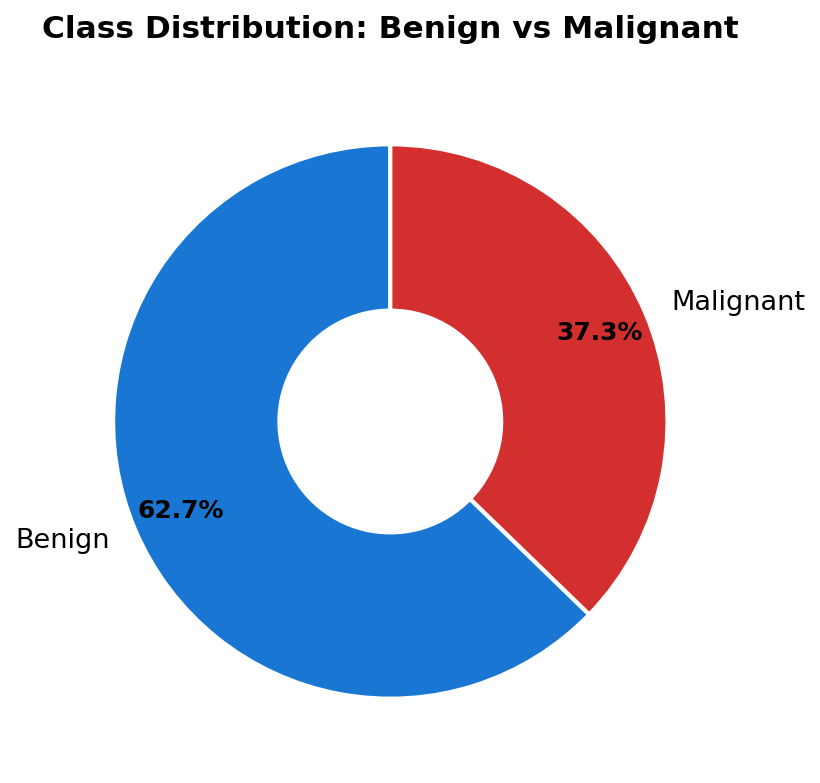
\includegraphics[width=0.52\textwidth]{public/images/class_distribution_pie.png}
  \caption{Class distribution: 357 Benign (62.7\%) and 212 Malignant (37.3\%) cases.
           The dataset is moderately imbalanced; this was accounted for by stratified
           train--test splitting.}
\end{figure}

%% ══════════════════════════════════════════════════════════════════════════
\section{Data Pre-processing}
%% ══════════════════════════════════════════════════════════════════════════

\subsection{Missing Value Check}
A systematic check confirmed \textbf{zero missing values} across all 30 features. No
imputation step was required.

\subsection{Feature Scaling --- StandardScaler}
\textbf{Why:} Features span vastly different scales (e.g.\ area ranges 143--2501
\textmu m$^2$, smoothness 0.05--0.16). Distance-based algorithms (kNN, DBSCAN, SVM with
RBF kernel) compute Euclidean distances, which are dominated by high-magnitude features
without scaling. $k$-Means computes centroid distances, again sensitive to scale.
Unscaled data would bias all four algorithms towards high-magnitude features.

\textbf{How:} Each feature $x_j$ was transformed to
\[
  \hat{x}_j = \frac{x_j - \mu_j}{\sigma_j}
\]
where $\mu_j$ and $\sigma_j$ are the feature mean and standard deviation estimated
\emph{on the training set only}, then applied to both train and test sets to prevent
data leakage.

\textbf{What changed:} All 30 features now have zero mean and unit variance. The
relative ordering of values within each feature is preserved; only their magnitude
and shift change.

\subsection{Train--Test Split}
The dataset was split into \textbf{80\% training} (455 samples) and \textbf{20\% test}
(114 samples) using stratified splitting (parameter \texttt{stratify=y}) to preserve
the original class ratio in both partitions, avoiding the pitfall of an over-represented
class in either split.

\subsection{After Pre-processing}

\begin{table}[H]
  \centering
  \caption{Dataset partitions after pre-processing}
  \begin{tabular}{lccc}
    \toprule
    \textbf{Split} & \textbf{Samples} & \textbf{Benign} & \textbf{Malignant} \\
    \midrule
    Training set & 455 & 286 & 169 \\
    Test set     & 114 &  71 &  43 \\
    \midrule
    Total        & 569 & 357 & 212 \\
    \bottomrule
  \end{tabular}
\end{table}

%% ══════════════════════════════════════════════════════════════════════════
\section{Statistical Analysis and Preliminary Exploration}
%% ══════════════════════════════════════════════════════════════════════════

\subsection{Descriptive Statistics}
Table~\ref{tab:stats} provides descriptive statistics for six representative features
before scaling.

\begin{table}[H]
  \centering
  \caption{Descriptive statistics for six key features (raw, unscaled values)}
  \label{tab:stats}
  \small
  \begin{tabular}{lrrrrrr}
    \toprule
    \textbf{Feature} & \textbf{Mean} & \textbf{Std} & \textbf{Min} & \textbf{Q1} & \textbf{Median} & \textbf{Max} \\
    \midrule
    Mean Radius      & 14.13 &  3.52 &  6.98 & 11.70 & 13.37 & 28.11 \\
    Mean Texture     & 19.29 &  4.30 &  9.71 & 16.17 & 18.84 & 39.28 \\
    Mean Perimeter   & 91.97 & 24.30 & 43.79 & 75.17 & 86.24 & 188.5 \\
    Mean Area        & 654.9 & 351.9 & 143.5 & 420.3 & 551.1 & 2501.0 \\
    Mean Smoothness  &  0.096 & 0.014 &  0.053 &  0.086 &  0.096 &  0.163 \\
    Mean Concavity   &  0.089 & 0.080 &  0.000 &  0.030 &  0.061 &  0.427 \\
    \bottomrule
  \end{tabular}
\end{table}

\subsection{Feature Distributions}

\begin{figure}[H]
  \centering
  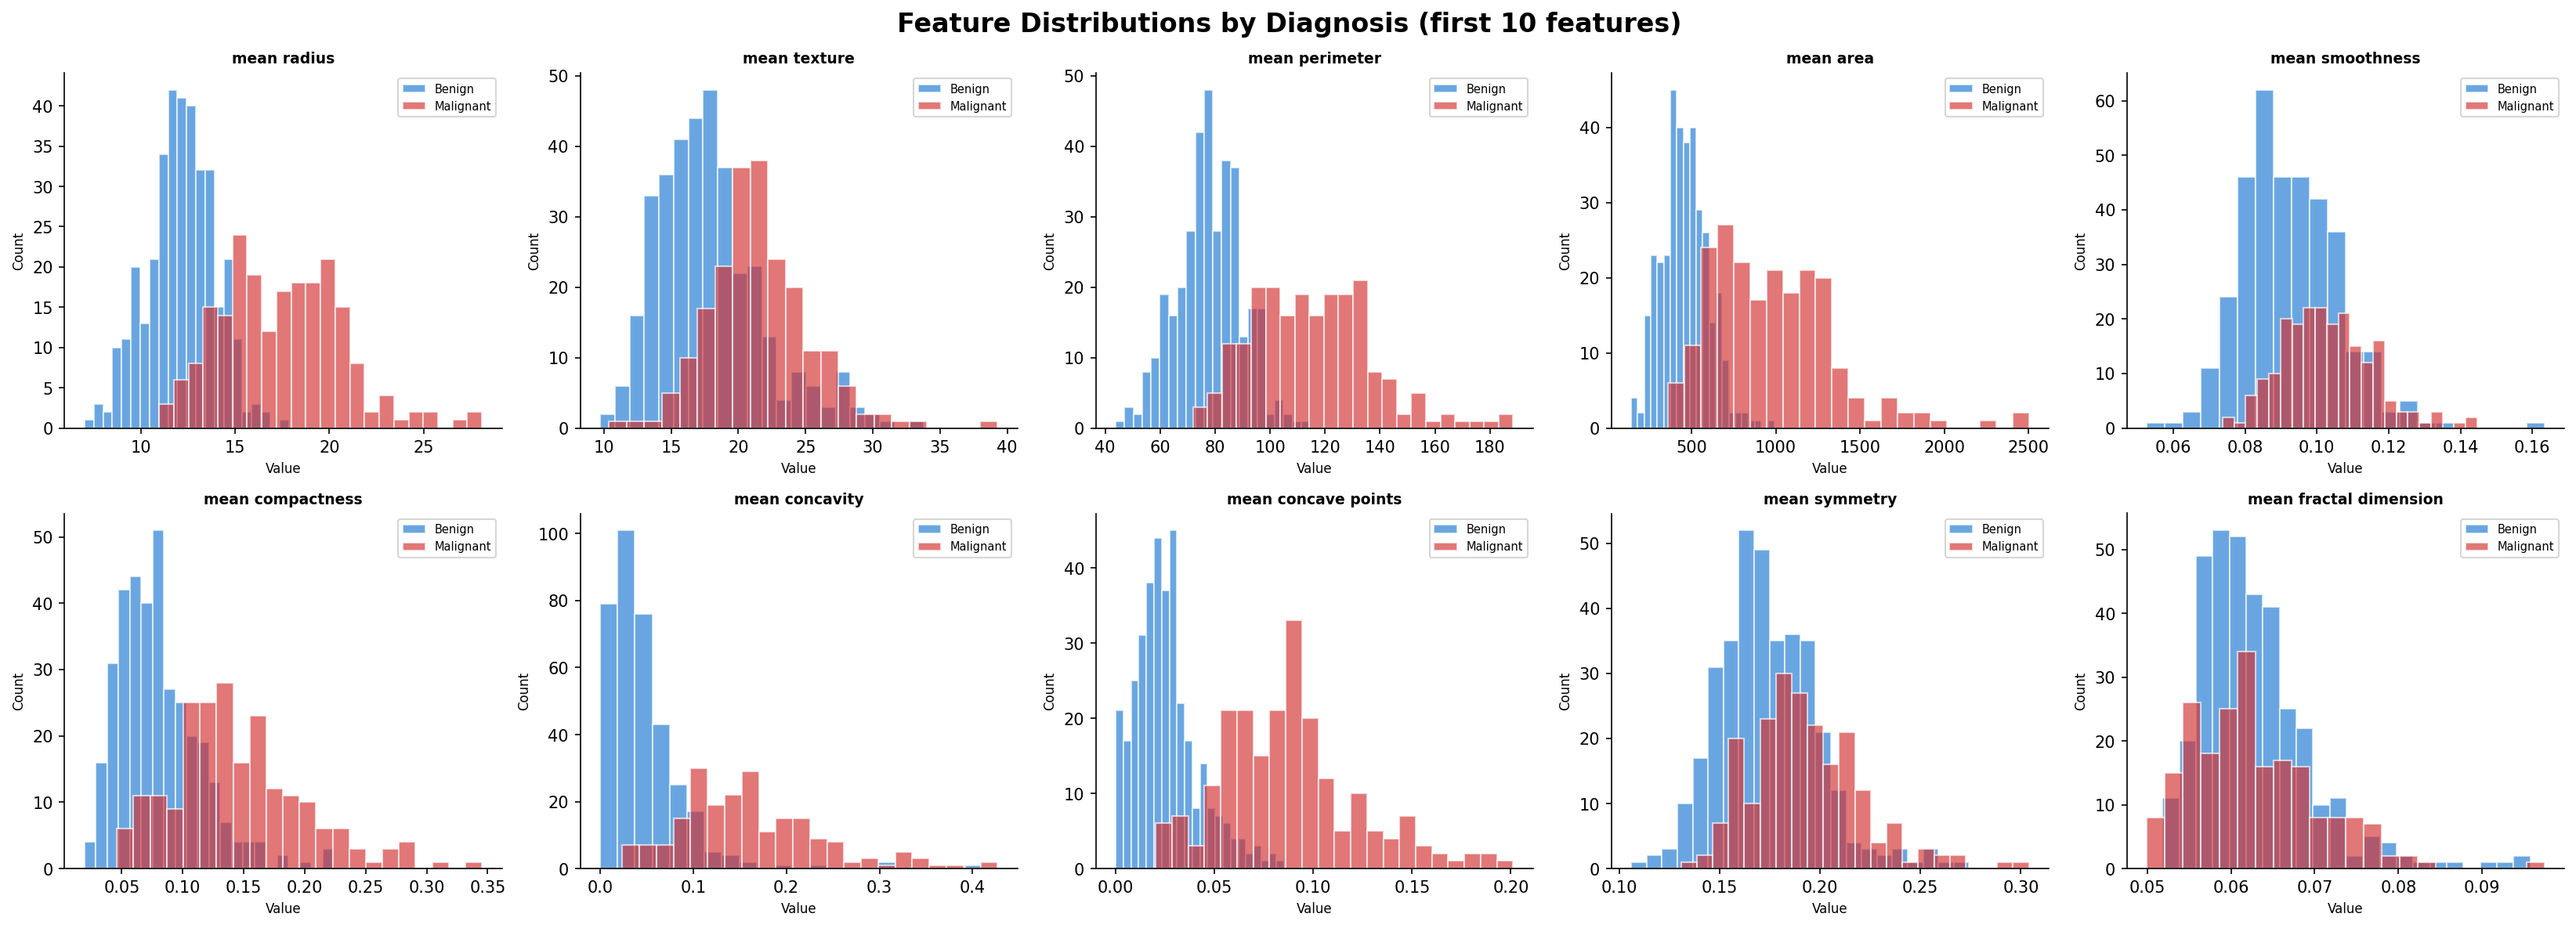
\includegraphics[width=\textwidth]{public/images/feature_distributions.png}
  \caption{Histograms of the first 10 features, split by diagnosis.
           Malignant cases (red) consistently show larger values for size-related
           features (radius, perimeter, area) and higher concavity.  Texture and
           smoothness distributions show greater overlap.}
\end{figure}

\textbf{Inference:} Morphological size features (radius, perimeter, area) are the most
discriminative: malignant nuclei are consistently larger and more irregular.  Texture
and smoothness are less separable, suggesting they contribute as complementary
rather than primary discriminants.

\subsection{Feature Correlation}

\begin{figure}[H]
  \centering
  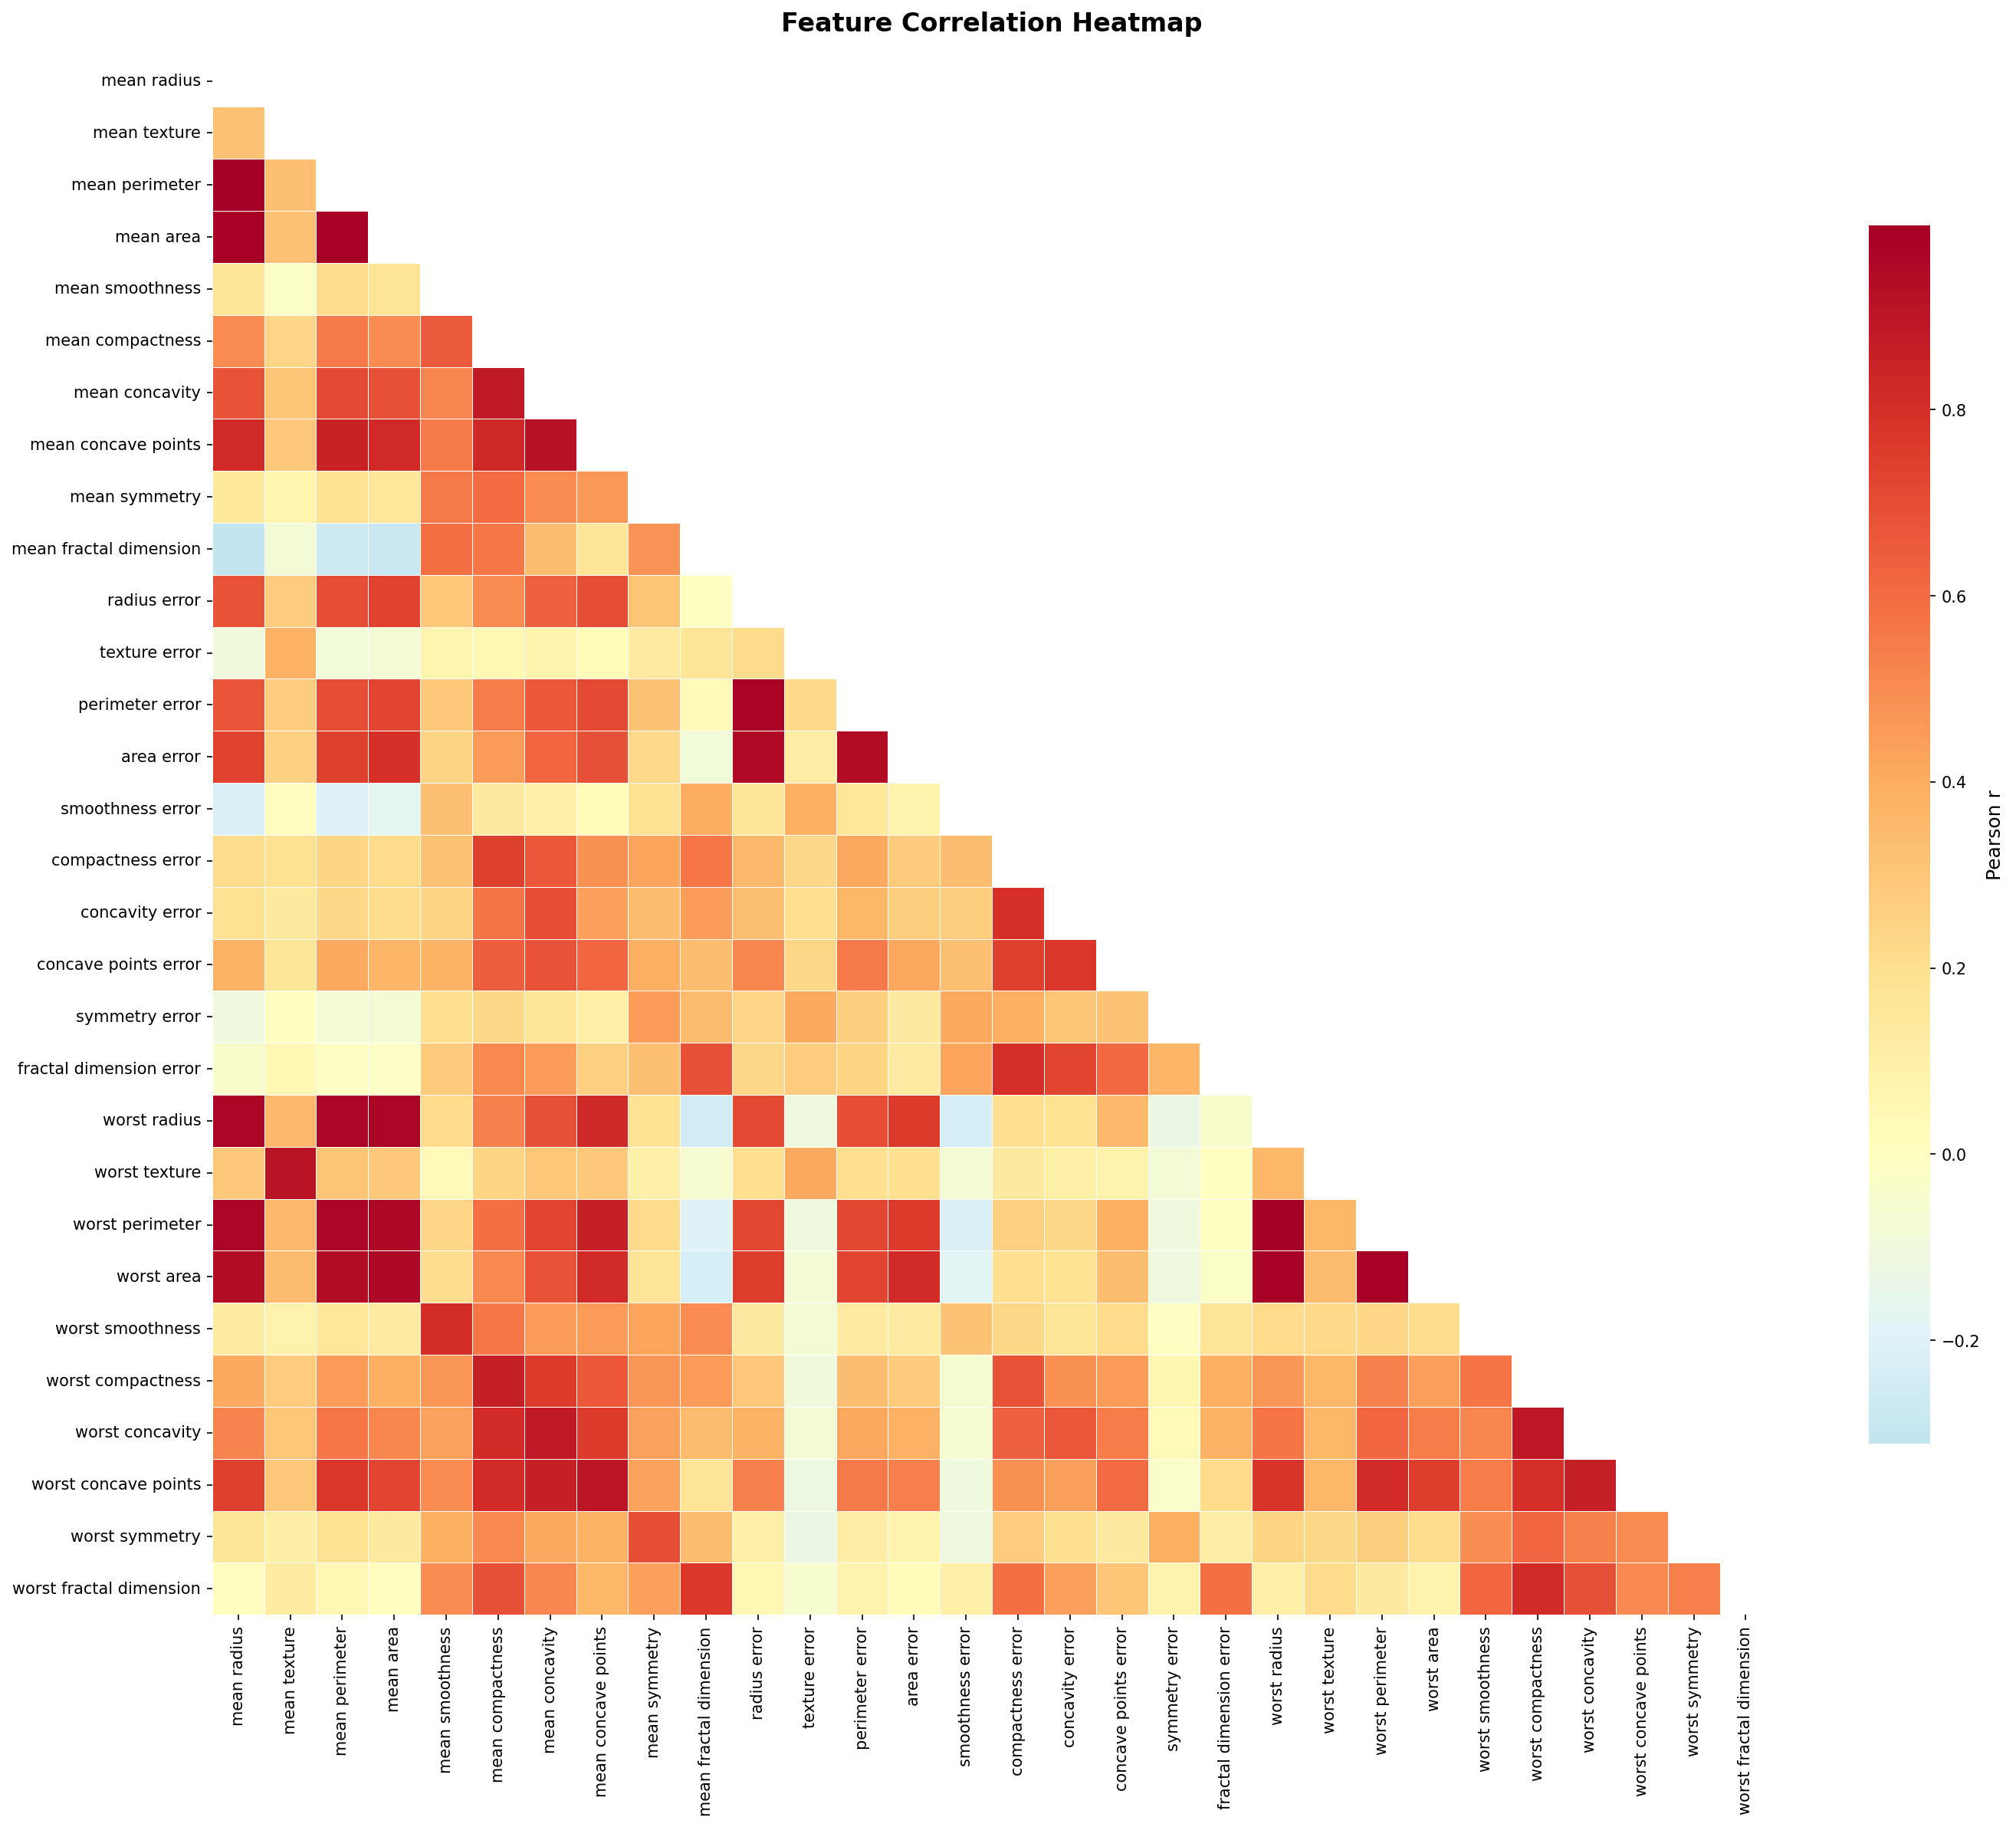
\includegraphics[width=0.98\textwidth]{public/images/correlation_heatmap.png}
  \caption{Lower-triangular Pearson correlation heatmap of all 30 features.
           Deep red regions indicate strong positive correlation; deep blue, strong
           negative correlation.  Size-related features (radius, perimeter, area,
           concave points) form a highly correlated cluster ($r > 0.9$).}
\end{figure}

\textbf{Inference:} The strong multicollinearity among size-related features explains
why even a small subset of features can achieve high classification accuracy.
SVM with an RBF kernel is not adversely affected by correlated inputs, while kNN
benefits from the scaling step that equalises their influence.

\subsection{Box Plots and Violin Plots}

\begin{figure}[H]
  \centering
  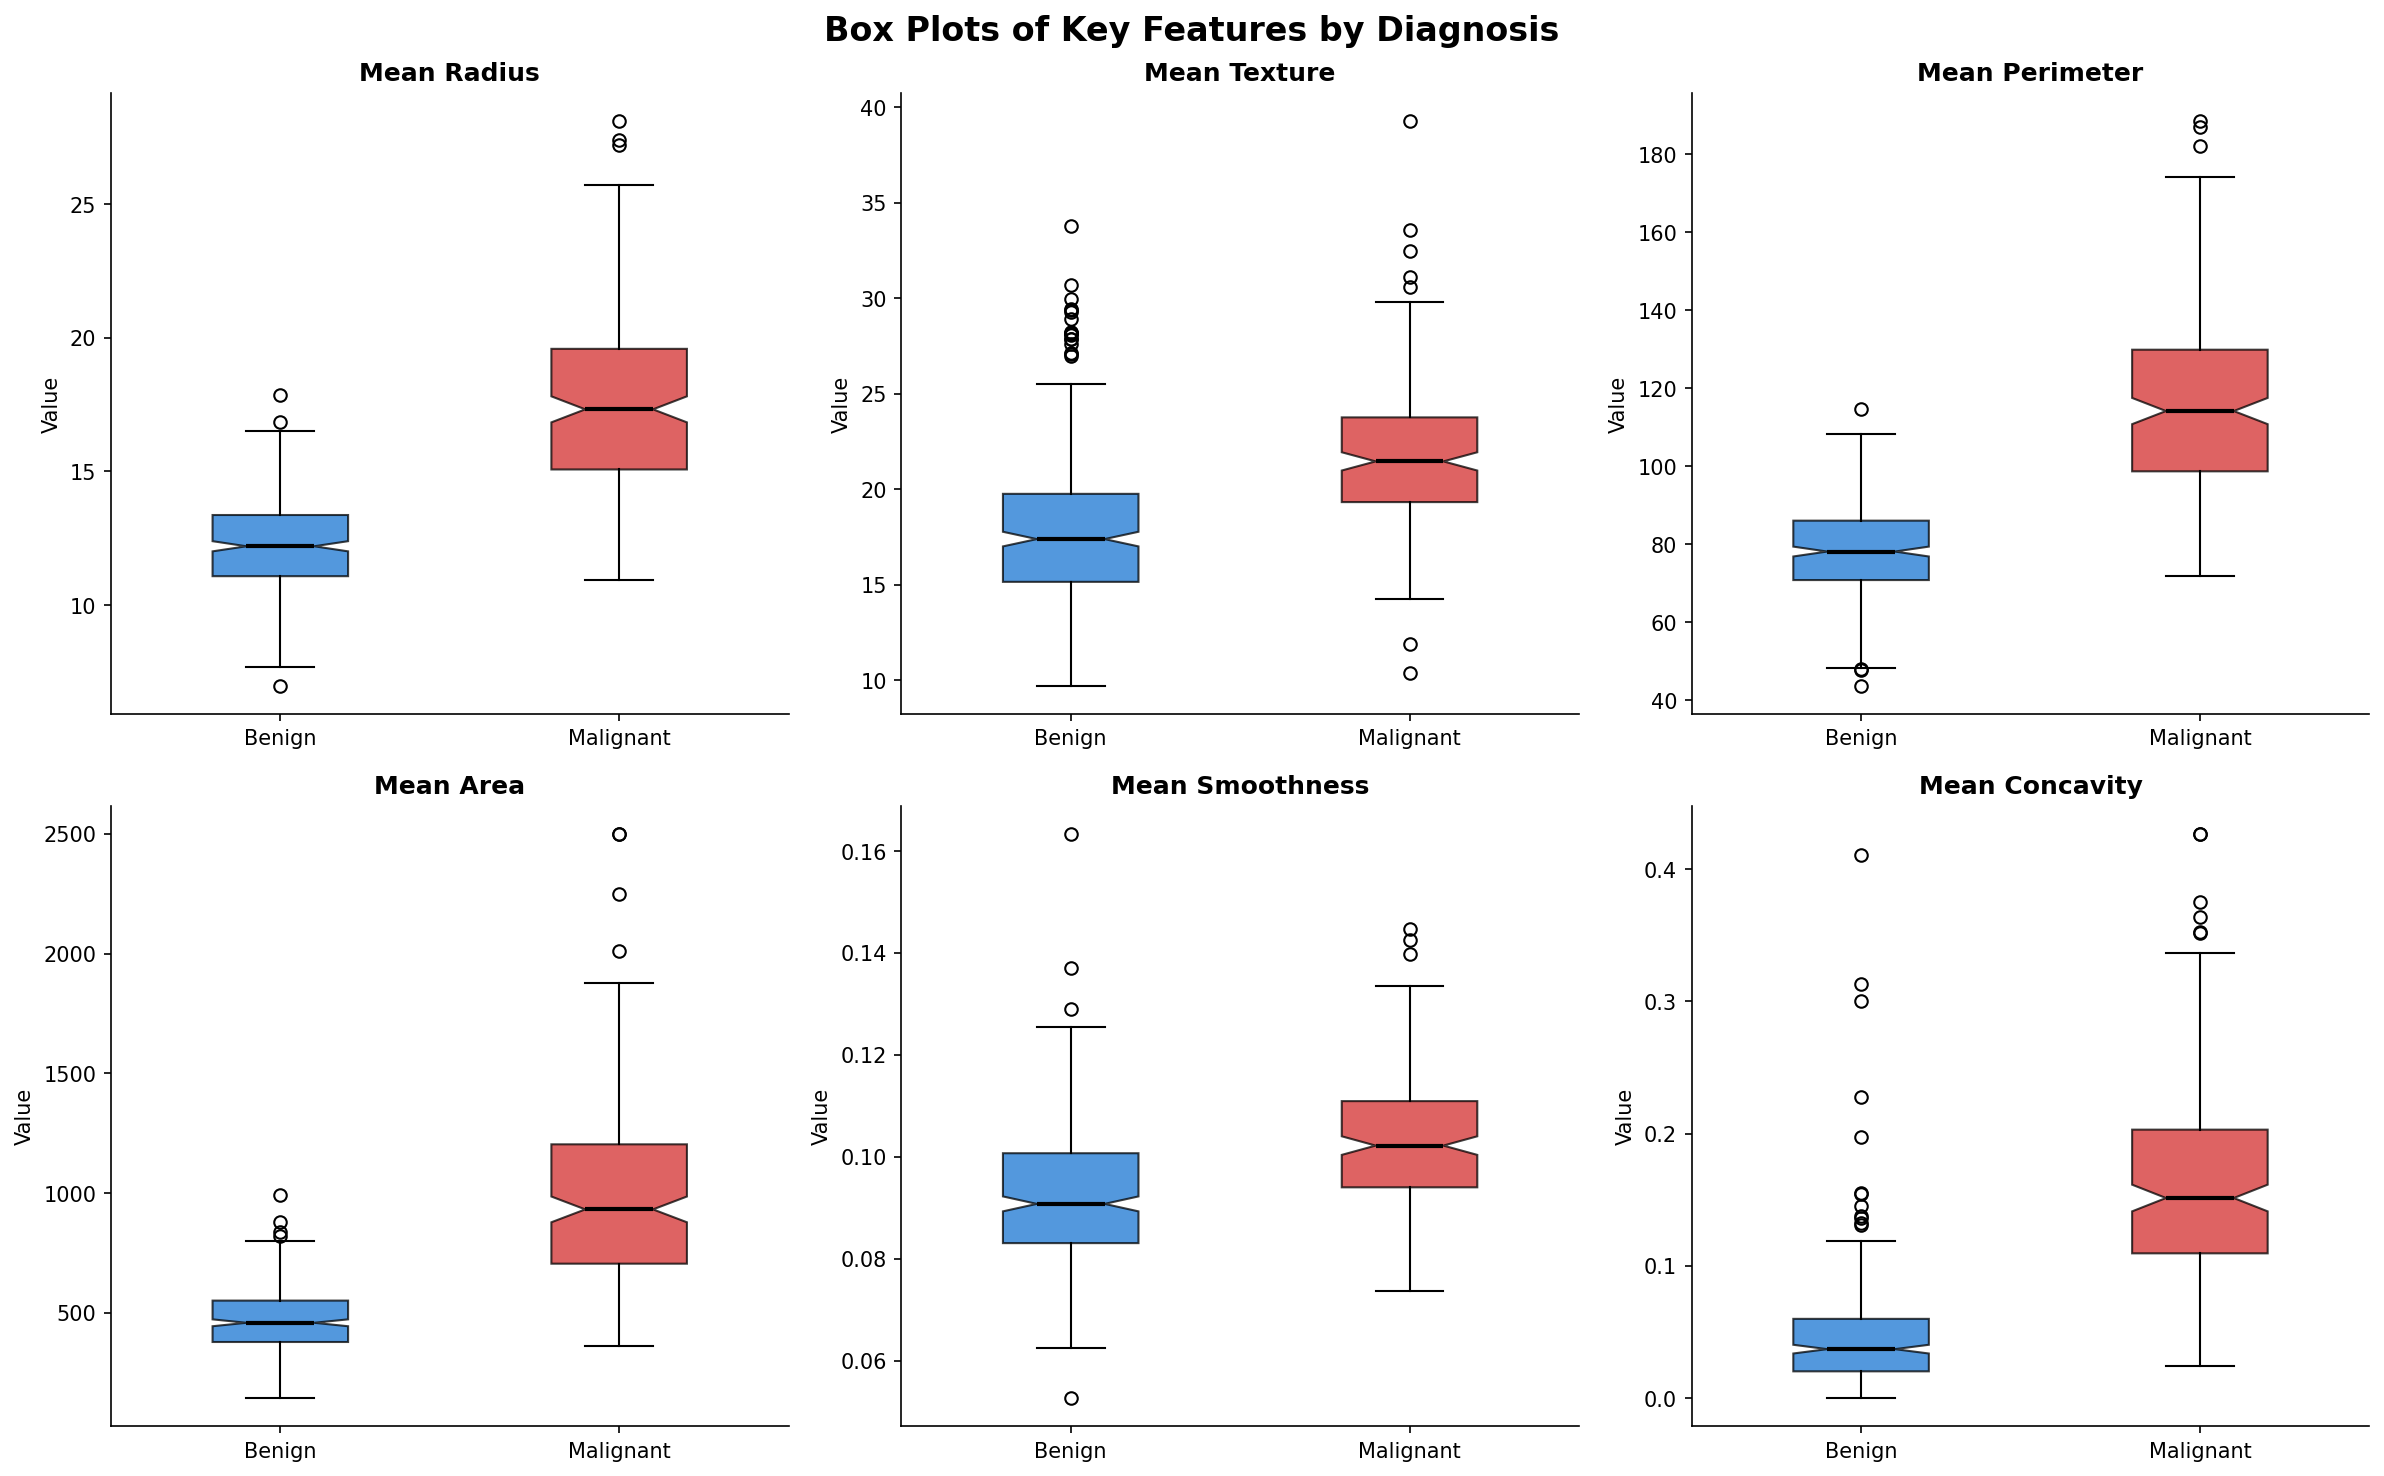
\includegraphics[width=\textwidth]{public/images/boxplot_features.png}
  \caption{Notched box plots comparing six key features between Benign and Malignant
           classes.  Non-overlapping notches indicate statistically significant
           differences in medians.  All six features show clear separation.}
\end{figure}

\begin{figure}[H]
  \centering
  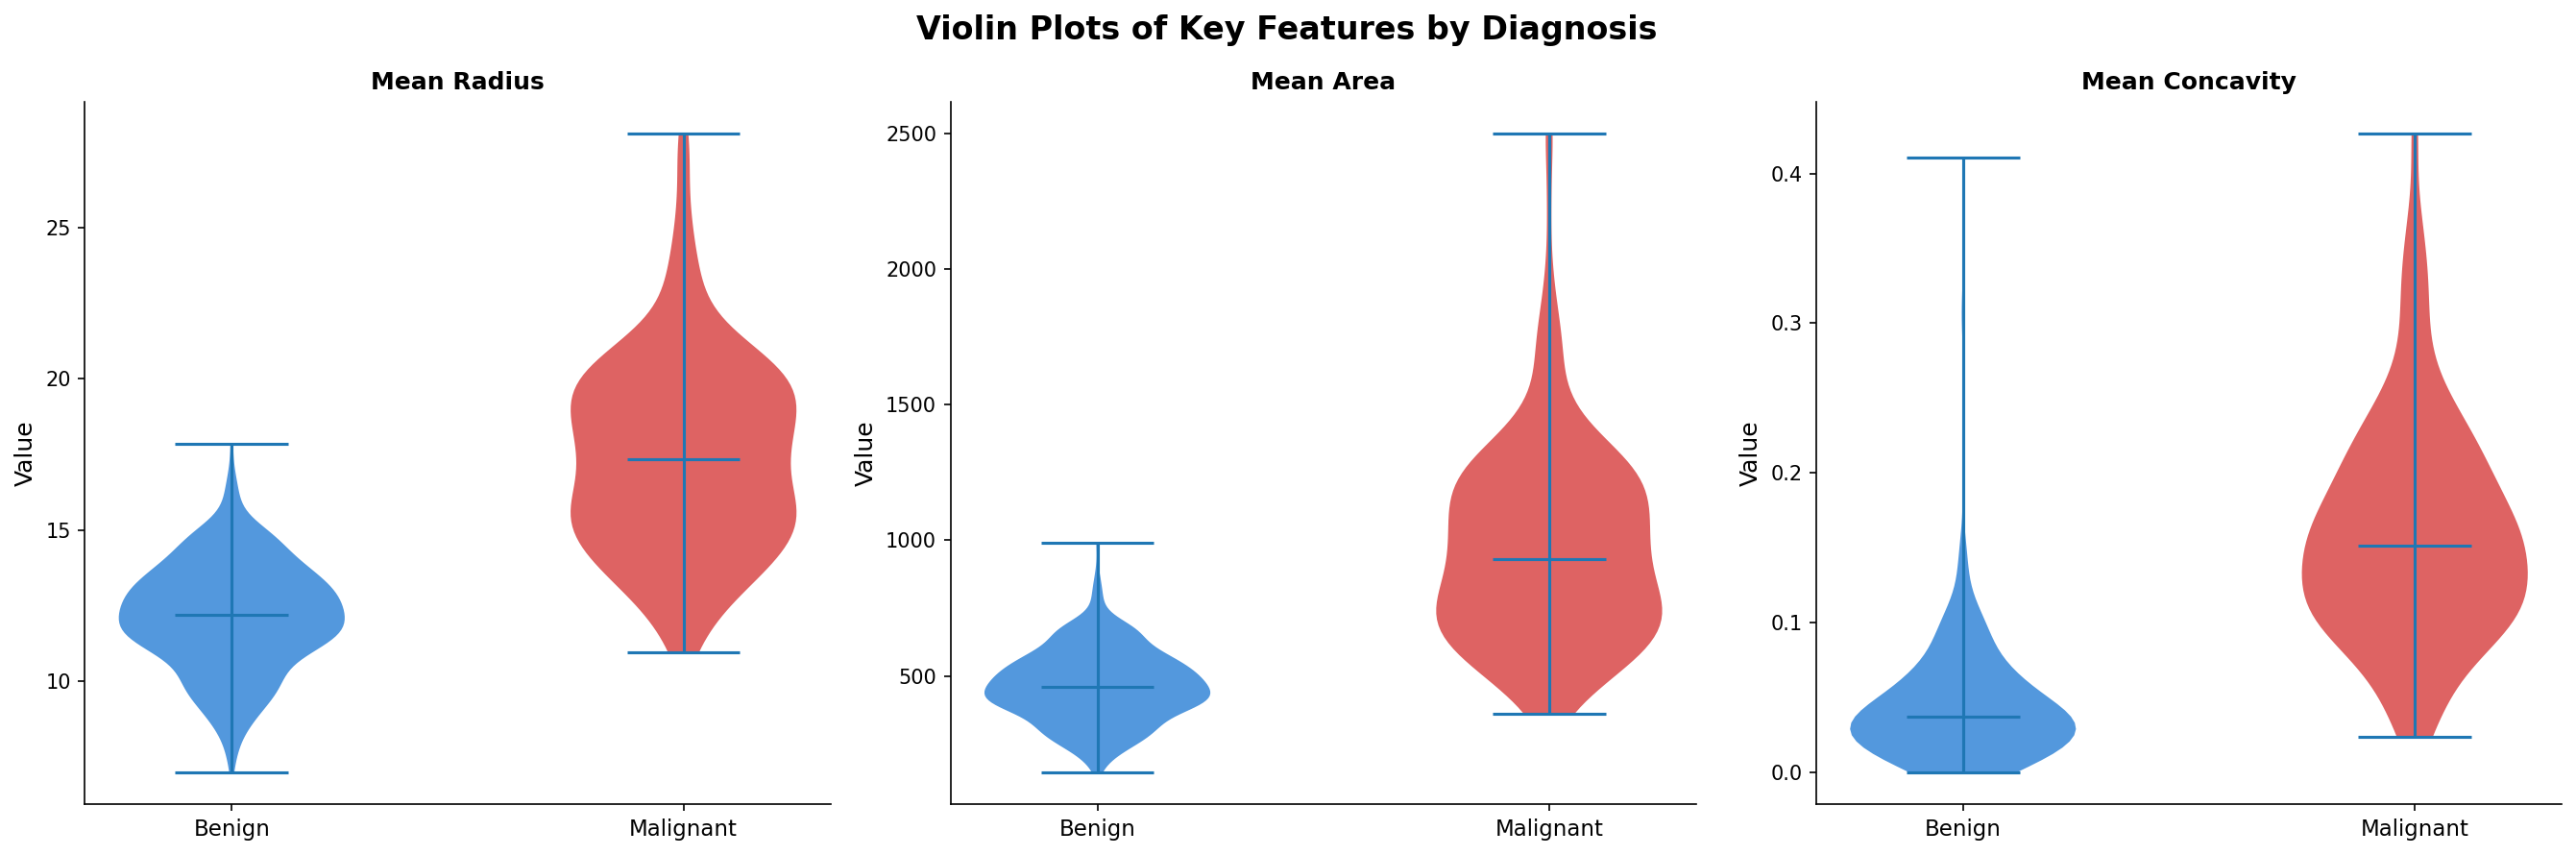
\includegraphics[width=\textwidth]{public/images/violin_plots.png}
  \caption{Violin plots for mean radius, area, and concavity.
           The bimodal shape visible in malignant concavity indicates a subgroup of
           highly irregular malignant tumours, which may represent a more aggressive
           subtype.}
\end{figure}

\begin{figure}[H]
  \centering
  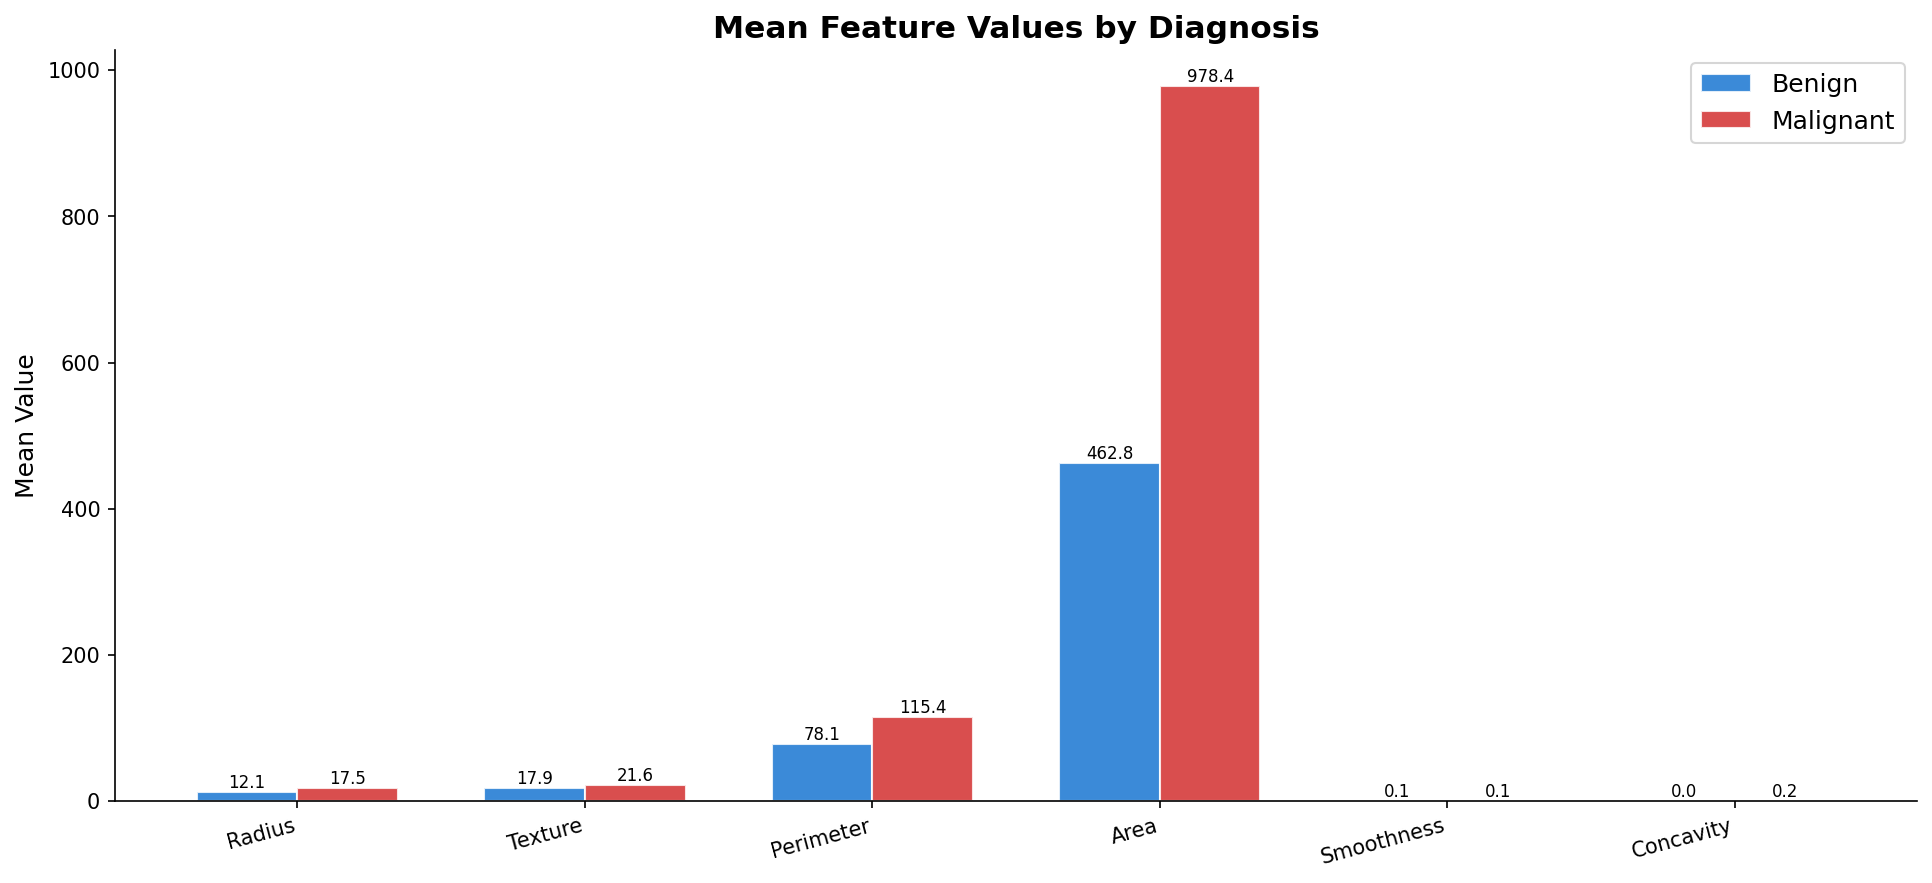
\includegraphics[width=\textwidth]{public/images/mean_feature_comparison.png}
  \caption{Mean feature values by diagnosis for six key features.  Malignant cases
           show 2--3$\times$ higher mean radius, perimeter, and area compared to
           benign cases, confirming that nuclear size is the dominant diagnostic
           marker.}
\end{figure}

\textbf{Key questions the analysis addresses:}
\begin{itemize}[leftmargin=2em]
  \item \textit{Q: Which features are the strongest discriminants?}
        A: Mean radius, perimeter, and area; followed by mean concavity and
        concave points.
  \item \textit{Q: Are there outliers that could distort ML models?}
        A: Yes, particularly in mean area (max 2501 vs.\ median 551); StandardScaler
        reduces but does not eliminate their influence, which is acceptable for SVM and
        kNN.
  \item \textit{Q: Is the dataset linearly separable?}
        A: The significant overlap in some features (texture, smoothness) suggests
        non-linear boundaries are beneficial, motivating the RBF kernel for SVM.
\end{itemize}

%% ══════════════════════════════════════════════════════════════════════════
\section{ML Classification}
%% ══════════════════════════════════════════════════════════════════════════

\subsection{Methodology}

\subsubsection{Support Vector Machine (SVM)}
SVM finds a maximum-margin hyperplane that separates the two classes in a
(possibly high-dimensional) feature space defined by a kernel function.  We used the
\textbf{Radial Basis Function (RBF) kernel}:
\[
  K(\mathbf{x}_i, \mathbf{x}_j) = \exp\!\left(-\gamma \|\mathbf{x}_i - \mathbf{x}_j\|^2\right)
\]
with $C{=}1.0$ and $\gamma{=}\texttt{scale}$ ($=1/(\text{n\_features} \times \sigma^2_X)$).

\textbf{Why RBF SVM?}  The feature distributions and correlation heatmap indicate that
the classes are not perfectly linearly separable (especially for texture and smoothness).
The RBF kernel maps the data into an infinite-dimensional space where a linear
separator may exist, effectively capturing non-linear decision boundaries.  SVM is also
robust to the moderate class imbalance (63:37) because the soft-margin formulation
optimises the margin rather than simple error counts.

\subsubsection{$k$-Nearest Neighbours (kNN)}
kNN classifies a test point by majority vote among its $k$ nearest neighbours in
scaled feature space.  We used $k{=}5$ with Euclidean distance.

\textbf{Why kNN?}  kNN is a non-parametric method that makes no distributional
assumptions. With $k{=}5$ (odd to avoid ties), it balances bias and variance for
this dataset size.  The 5-fold cross-validation accuracy of 96.49\% on the full
scaled dataset confirms that $k{=}5$ is a robust choice.

\subsection{Evaluation Metrics}

\begin{itemize}[leftmargin=2em]
  \item \textbf{Accuracy}: fraction of correct predictions.
  \item \textbf{Cohen's $\kappa$}: agreement beyond chance
        ($\kappa = 0$ pure chance, $\kappa = 1$ perfect agreement).
  \item \textbf{ROC-AUC}: area under the Receiver Operating Characteristic curve;
        probability that the model ranks a random positive higher than a random
        negative.  AUC $= 1.0$ is perfect; AUC $= 0.5$ is random.
\end{itemize}

\subsection{Results}

\begin{table}[H]
  \centering
  \caption{Classification performance on the held-out test set (114 samples)}
  \label{tab:clf}
  \begin{tabular}{lcccc}
    \toprule
    \textbf{Algorithm} & \textbf{Accuracy} & \textbf{Cohen's $\kappa$} & \textbf{ROC-AUC} & \textbf{5-CV Accuracy} \\
    \midrule
    SVM (RBF, $C{=}1$) & \textbf{0.9825} & \textbf{0.9623} & \textbf{0.9950} & 0.9736 \\
    kNN ($k{=}5$)       & 0.9649          & 0.9238          & 0.9792          & \textbf{0.9649} \\
    \bottomrule
  \end{tabular}
\end{table}

\subsubsection{Confusion Matrices}

\begin{figure}[H]
  \centering
  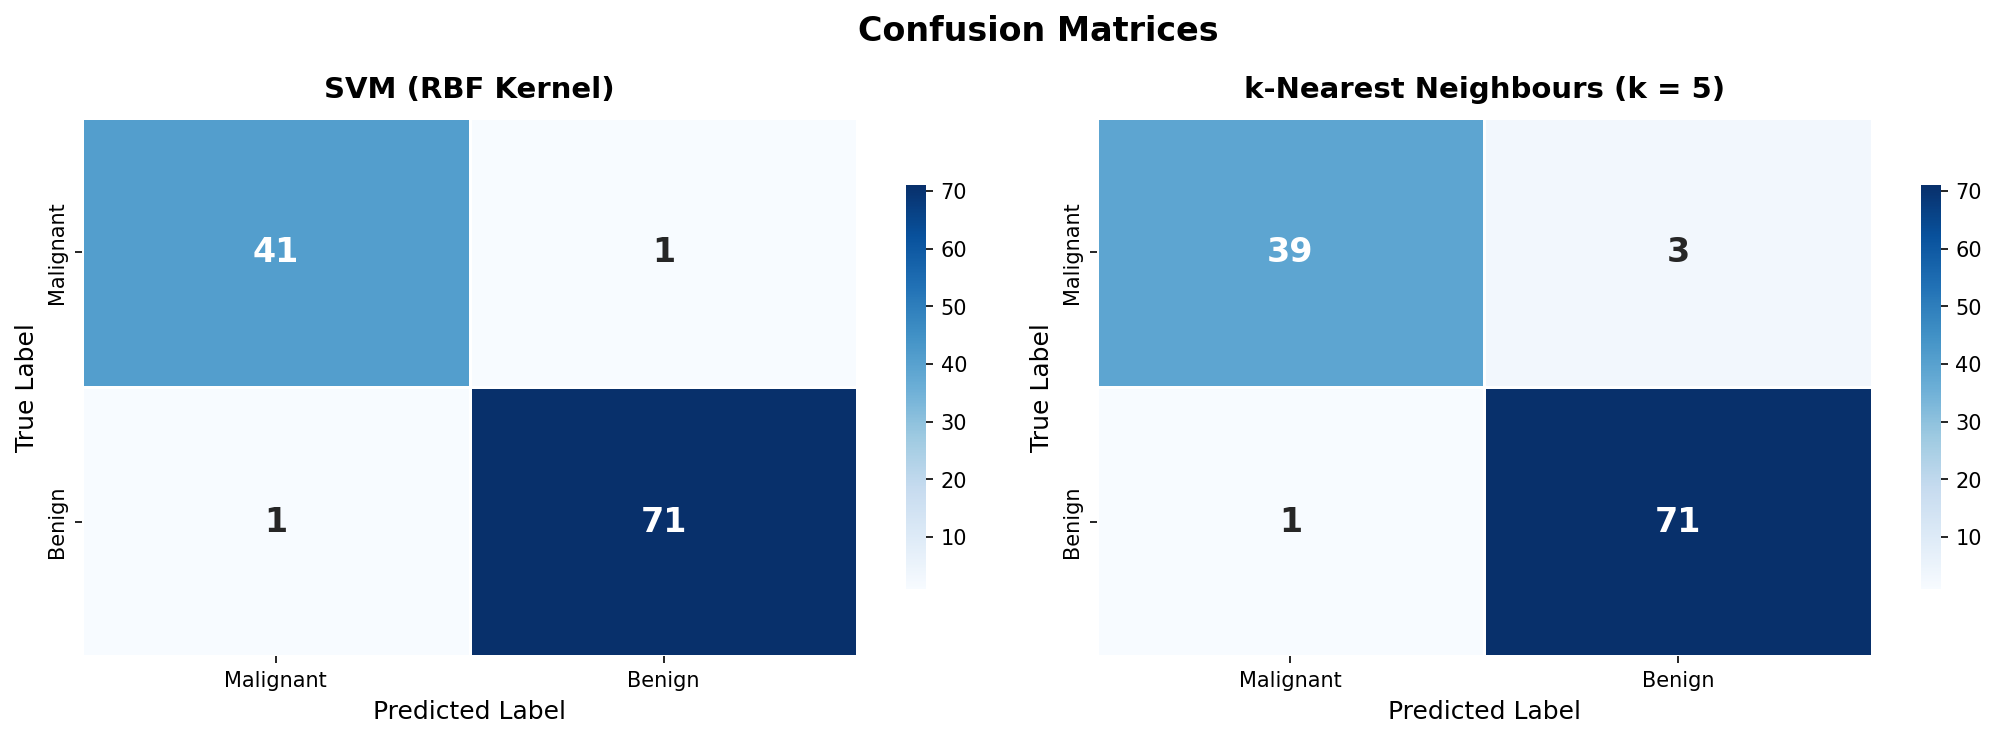
\includegraphics[width=\textwidth]{public/images/confusion_matrices.png}
  \caption{Confusion matrices for SVM (left) and kNN (right) on the 114-sample test
           set.  Both classifiers show high true-positive rates. SVM makes only
           2 total errors; kNN makes 4.  The clinically critical false-negative
           count (malignant classified as benign) is 1 for SVM and 3 for kNN.}
\end{figure}

\subsubsection{ROC Curves}

\begin{figure}[H]
  \centering
  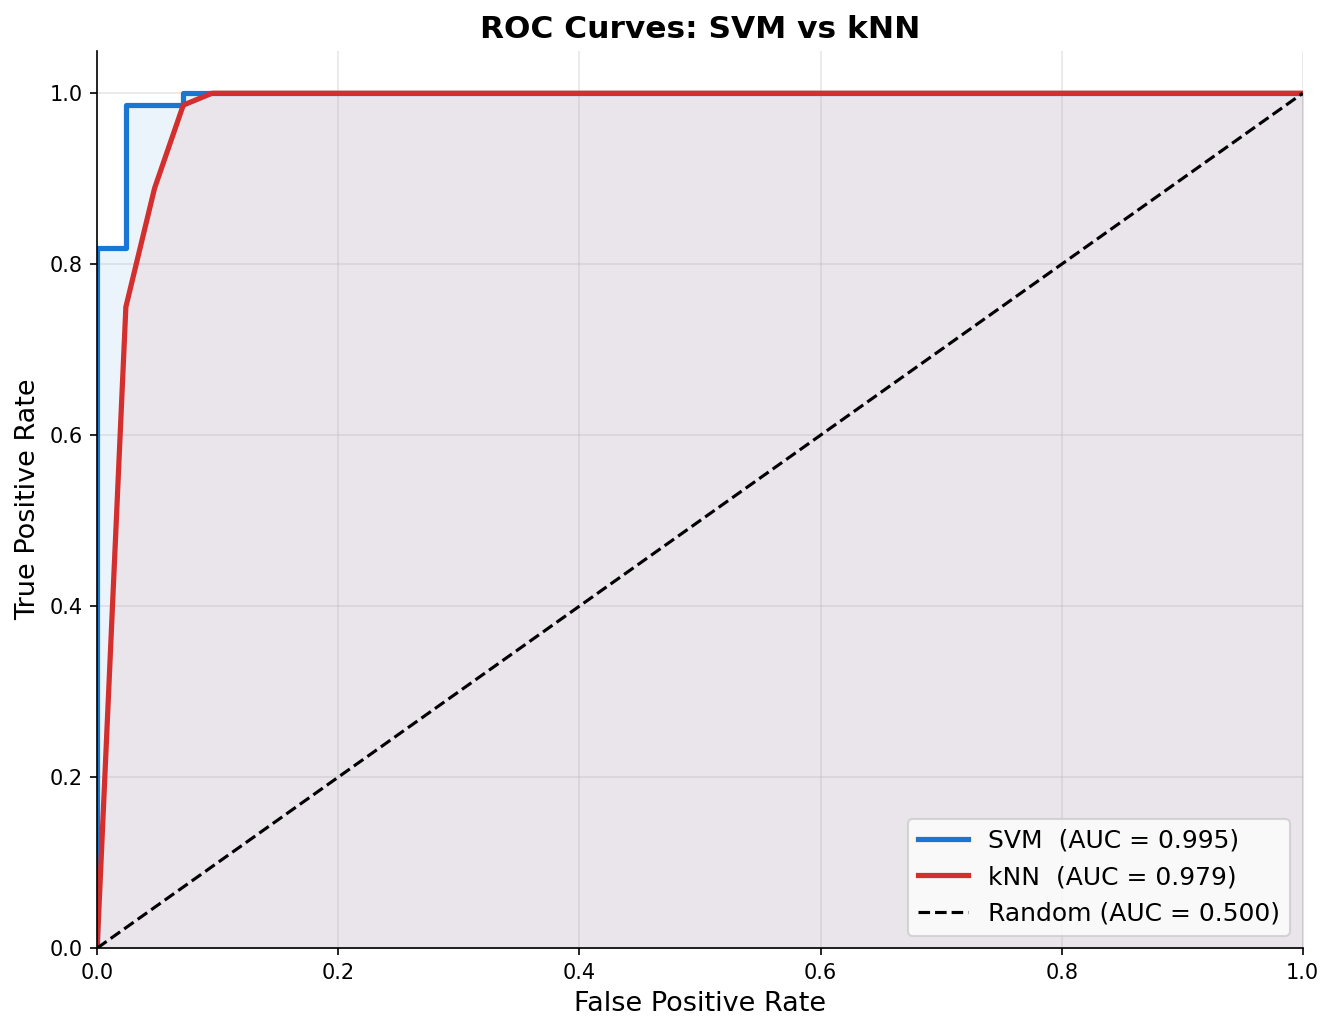
\includegraphics[width=0.80\textwidth]{public/images/roc_curves.png}
  \caption{ROC curves for SVM (AUC $= 0.995$) and kNN (AUC $= 0.979$).  Both
           curves are near the top-left corner, indicating excellent discrimination.
           SVM's curve is uniformly higher, confirming its superior probabilistic
           calibration.}
\end{figure}

\subsubsection{Metric Comparison}

\begin{figure}[H]
  \centering
  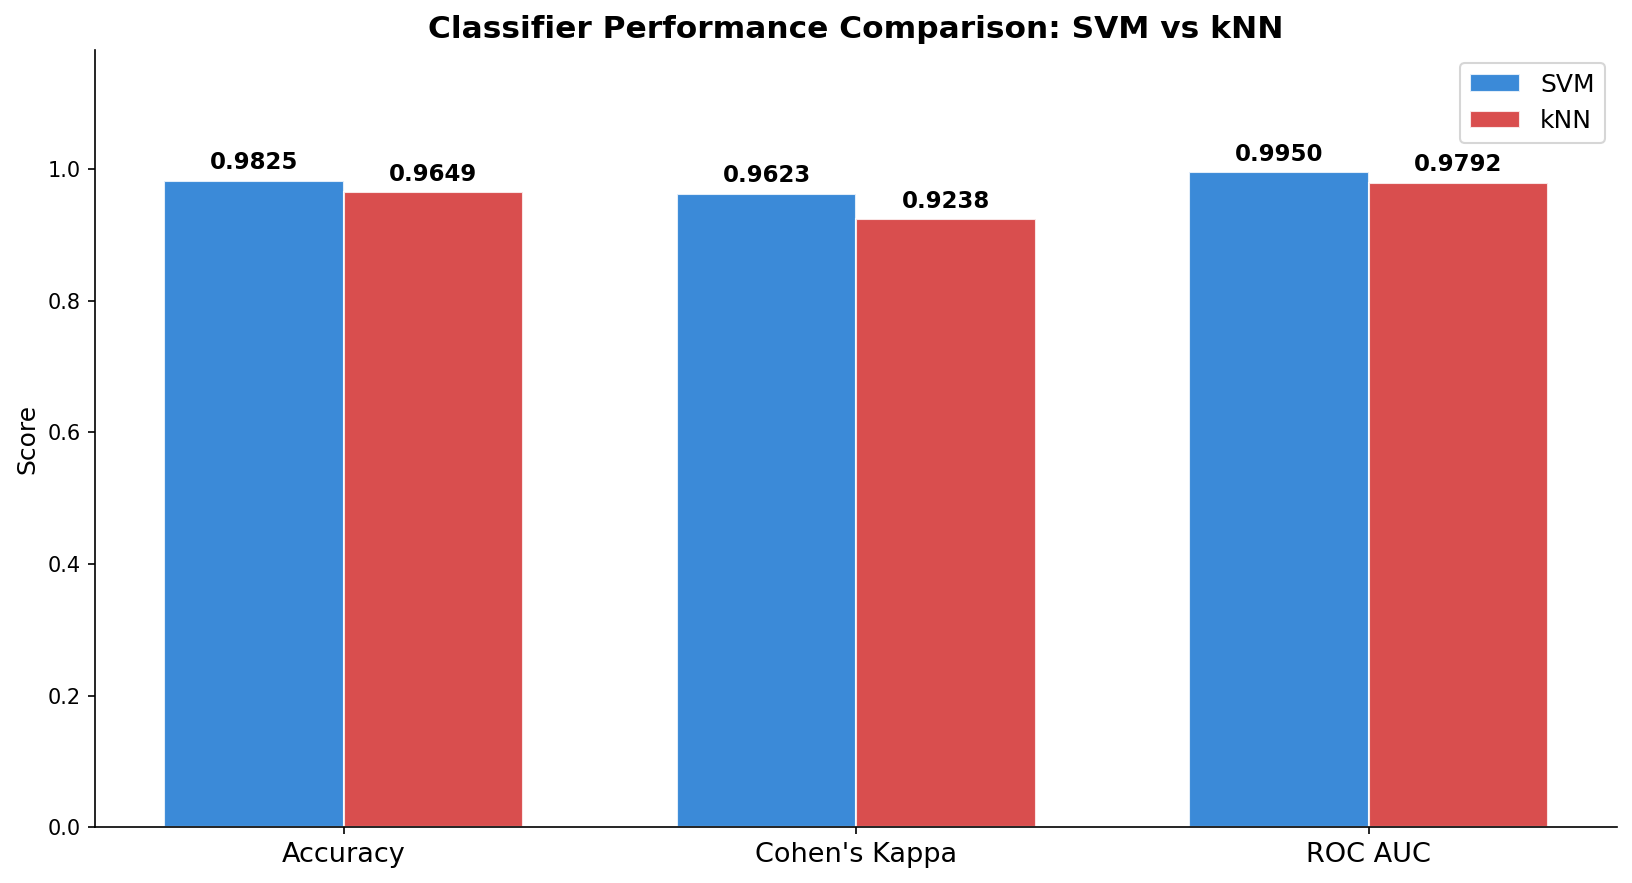
\includegraphics[width=0.90\textwidth]{public/images/classifier_comparison.png}
  \caption{Side-by-side bar chart comparing accuracy, Cohen's $\kappa$, and ROC-AUC
           for SVM and kNN.  SVM leads on all three metrics.}
\end{figure}

\subsection{Discussion and Inferences}

\begin{enumerate}[leftmargin=2em]
  \item \textbf{SVM outperforms kNN} on all metrics.  The RBF kernel exploits the
        non-linear structure noted in the preliminary analysis, while kNN, despite
        scaling, is affected by the high dimensionality (30 features) --- a manifestation
        of the curse of dimensionality.
  \item \textbf{Clinical significance of false negatives}: SVM produces only 1
        false negative (malignant predicted as benign) vs.\ 3 for kNN.  In a medical
        screening context, false negatives are the more dangerous error as they
        delay treatment.  SVM is therefore the preferred model for this application.
  \item \textbf{High Cohen's $\kappa$ values} ($>0.92$ for both) confirm that neither
        model is exploiting class imbalance --- both genuinely learn the discriminative
        structure of the data.
  \item A 5-fold cross-validation accuracy of 97.36\% for SVM confirms its
        generalisability beyond the specific train--test split.
\end{enumerate}

%% ══════════════════════════════════════════════════════════════════════════
\section{Clustering Analysis}
%% ══════════════════════════════════════════════════════════════════════════

\subsection{Methodology}

Clustering is applied \emph{without} using the class labels, allowing us to test
whether the natural geometric structure of the data recovers the clinical classes.
All clustering is performed on the StandardScaler-normalised full dataset
(569 samples, 30 features).  Results are visualised via PCA projection to 2D.

\subsubsection{$k$-Means}
$k$-Means partitions data into $k$ clusters by iteratively assigning points to the
nearest centroid and recomputing centroids until convergence.  It minimises intra-cluster
SSE (also called inertia):
\[
  \text{SSE} = \sum_{j=1}^{k} \sum_{\mathbf{x} \in C_j} \|\mathbf{x} - \boldsymbol{\mu}_j\|^2
\]
\textbf{Parameter choice:} We ran $k$-Means for $k = 2,\ldots,10$ and plotted the
elbow curve to identify the optimal $k$.

\subsubsection{DBSCAN}
DBSCAN (Density-Based Spatial Clustering of Applications with Noise) groups points
that are closely packed together and marks as noise points that lie in low-density
regions.  Key parameters: \texttt{eps} (neighbourhood radius) and
\texttt{min\_samples} (minimum points to form a core).

\textbf{Parameter choice:} After grid search on the scaled data, \texttt{eps}$=2.5$,
\texttt{min\_samples}$=5$ produced a meaningful partition.

\textbf{Why DBSCAN?}  Unlike $k$-Means, DBSCAN does not assume convex spherical
clusters, can find clusters of arbitrary shape, and explicitly identifies noise
(outlier) points.  It is parameter-sensitive but avoids forcing every point into a
cluster.

\subsection{Elbow Plot}

\begin{figure}[H]
  \centering
  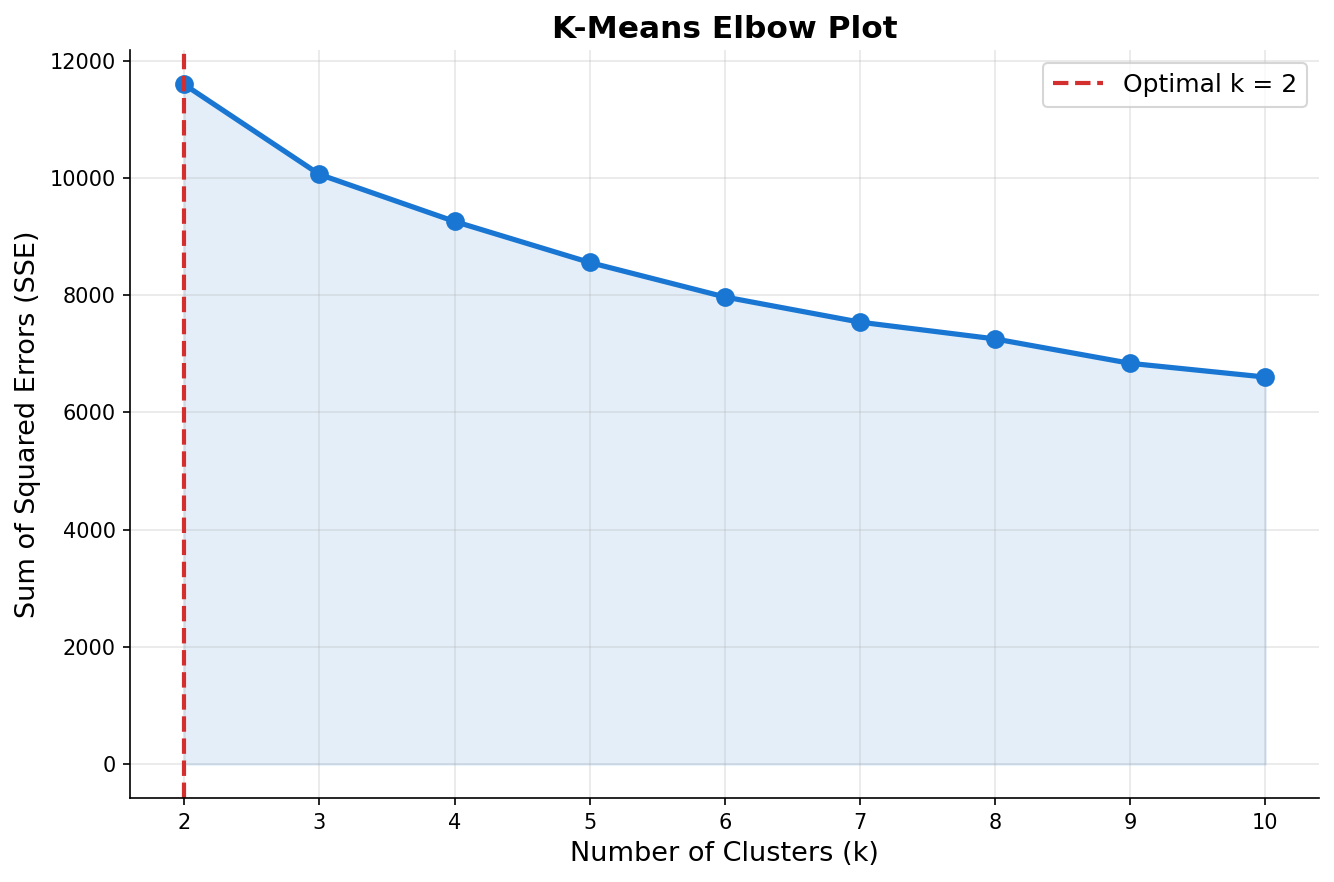
\includegraphics[width=0.78\textwidth]{public/images/elbow_plot.png}
  \caption{SSE (inertia) vs.\ number of clusters $k$ for $k$-Means.
           The sharpest bend occurs at $k{=}2$, consistent with the true number
           of clinical classes (Benign / Malignant).  Beyond $k{=}4$ the gains
           are marginal.}
\end{figure}

\subsection{K-Means Clustering Result ($k=2$)}

\begin{figure}[H]
  \centering
  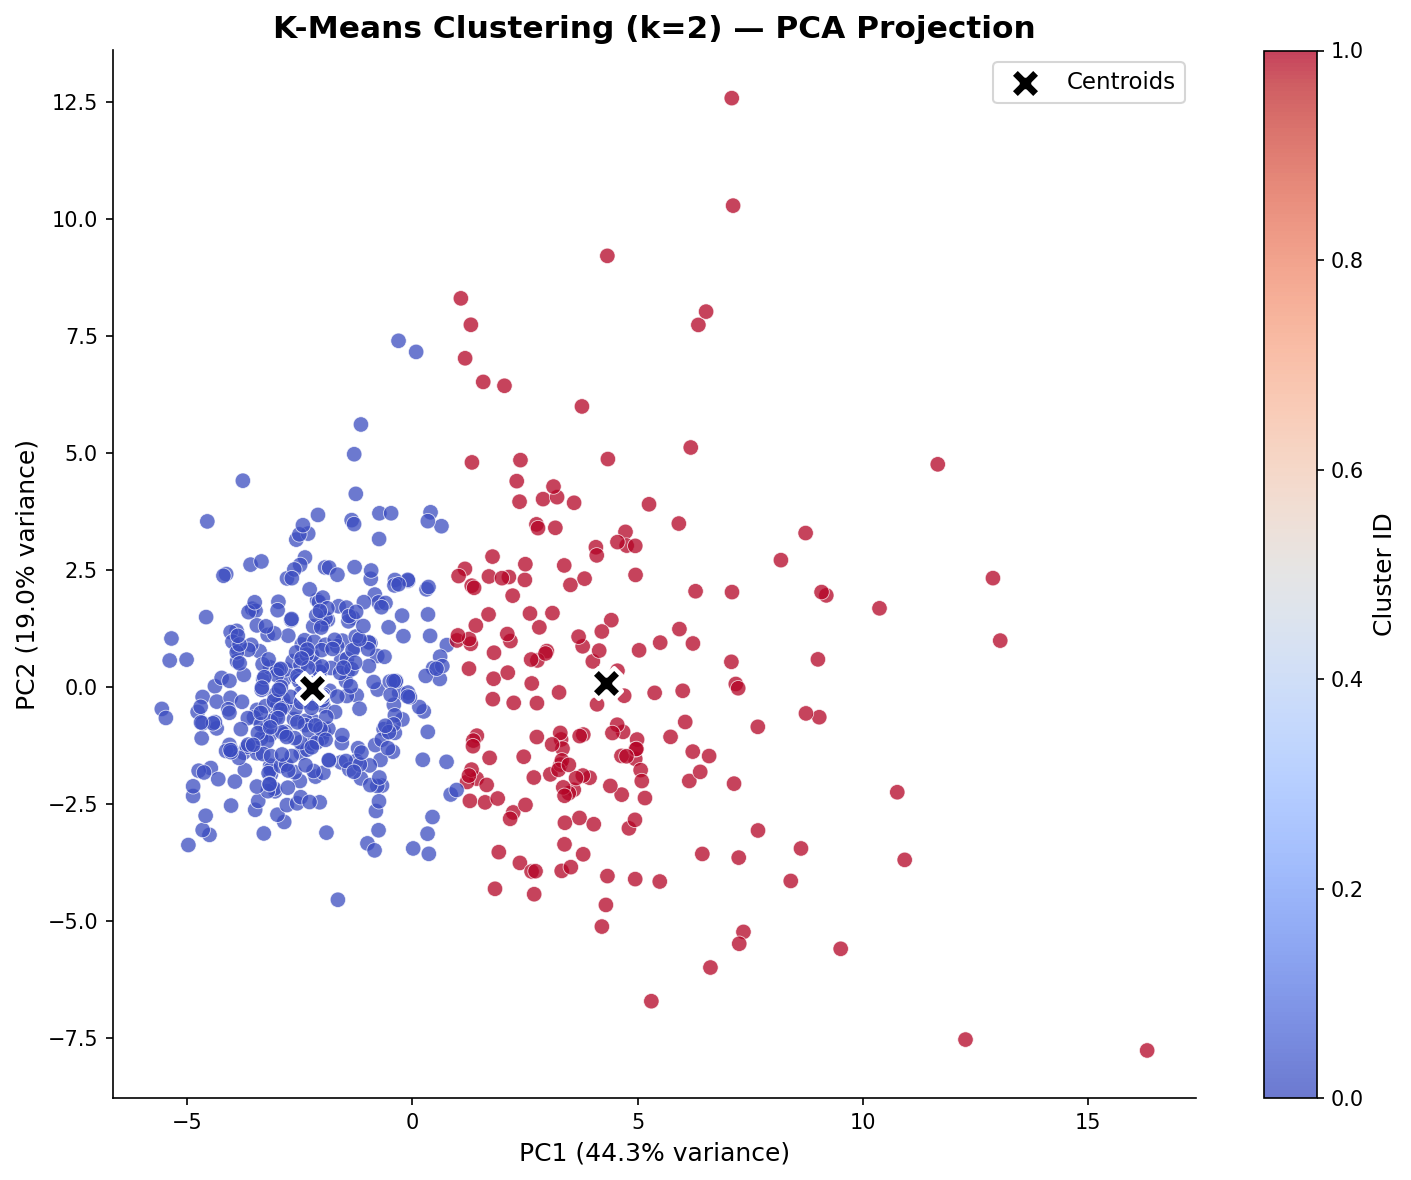
\includegraphics[width=0.82\textwidth]{public/images/kmeans_clusters.png}
  \caption{$k$-Means clusters ($k{=}2$) projected onto the first two principal
           components (PC1: 44.3\% variance, PC2: 19.0\% variance).  Black crosses
           mark cluster centroids.  The two clusters correspond closely to the
           Benign and Malignant classes, demonstrating that unsupervised geometry
           mirrors the clinical labels.}
\end{figure}

\subsection{DBSCAN Clustering Result}

\begin{figure}[H]
  \centering
  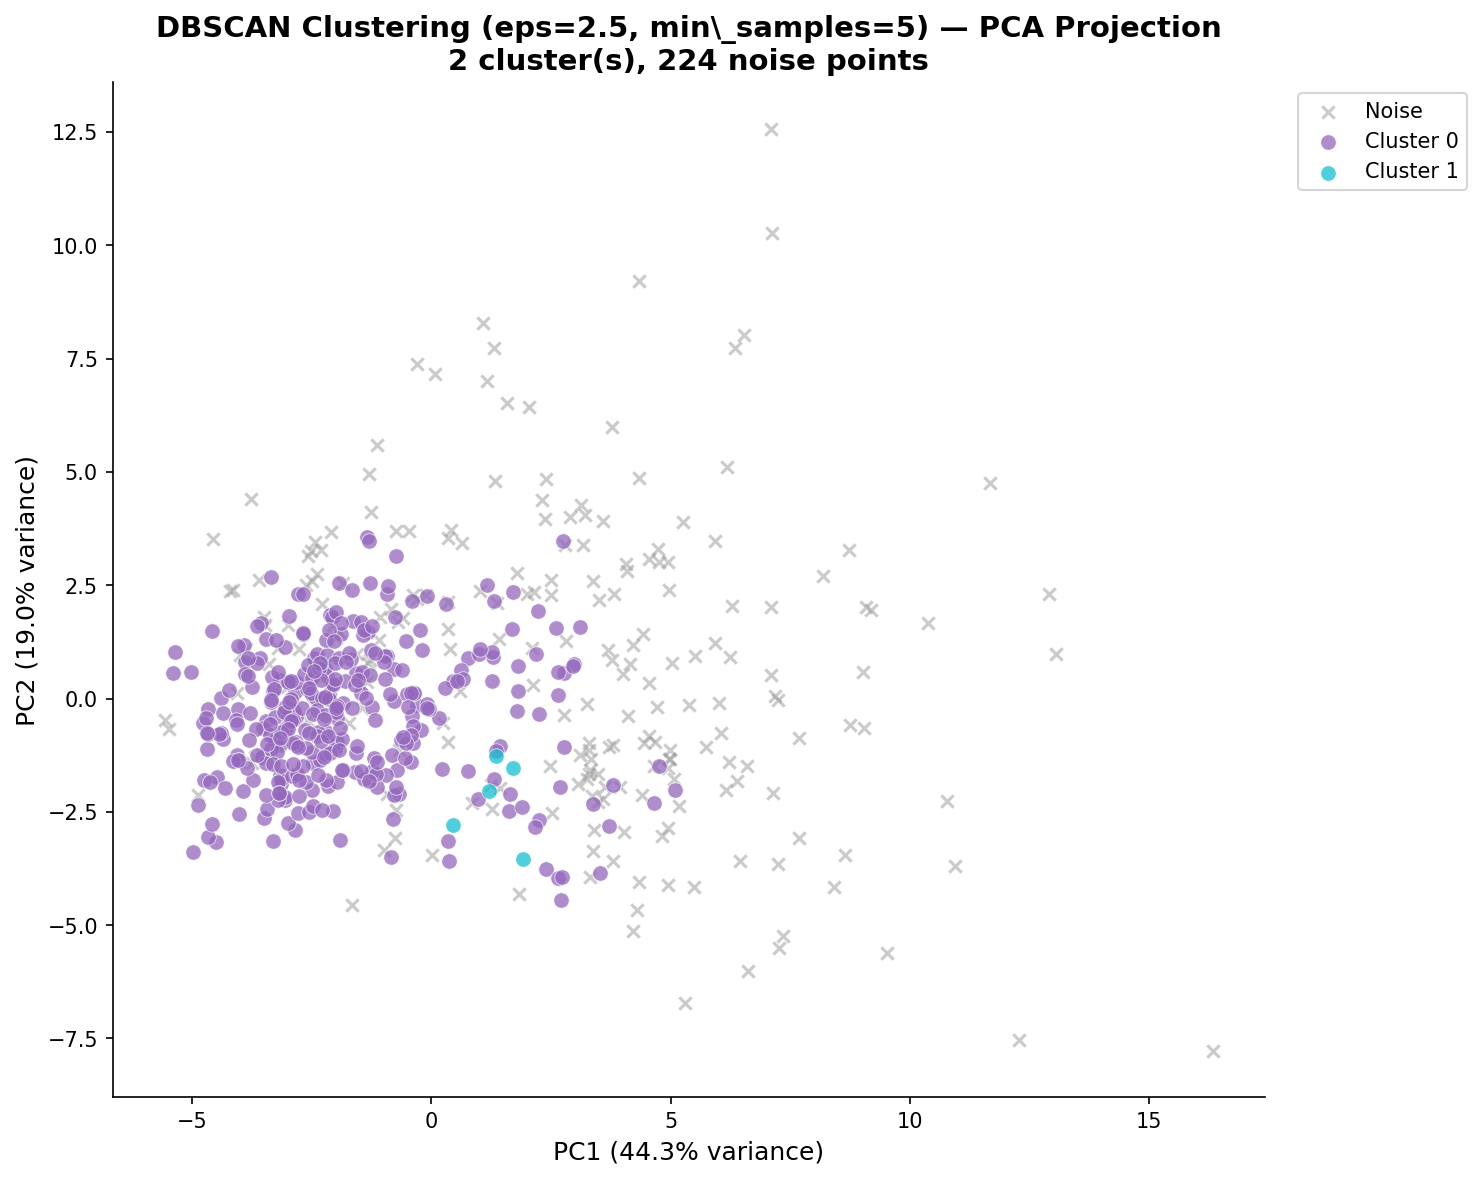
\includegraphics[width=0.88\textwidth]{public/images/dbscan_clusters.png}
  \caption{DBSCAN clusters (eps$=2.5$, min\_samples$=5$) on the PCA projection.
           DBSCAN identifies 2 main clusters and flags 224 points (39.4\%) as noise
           (grey crosses).  The high noise fraction reflects the fact that the breast
           cancer feature space has a broad, diffuse density rather than tight,
           well-separated clusters that DBSCAN excels at finding.}
\end{figure}

\subsection{Entropy and SSE Comparison}

\textbf{Entropy} measures class impurity within clusters:
\[
  H = -\sum_{j} \frac{|C_j|}{N} \sum_{c} p_{jc} \log_2 p_{jc}
\]
where $p_{jc}$ is the fraction of class $c$ in cluster $j$.
Lower entropy $\Rightarrow$ purer (more class-coherent) clusters.

\begin{figure}[H]
  \centering
  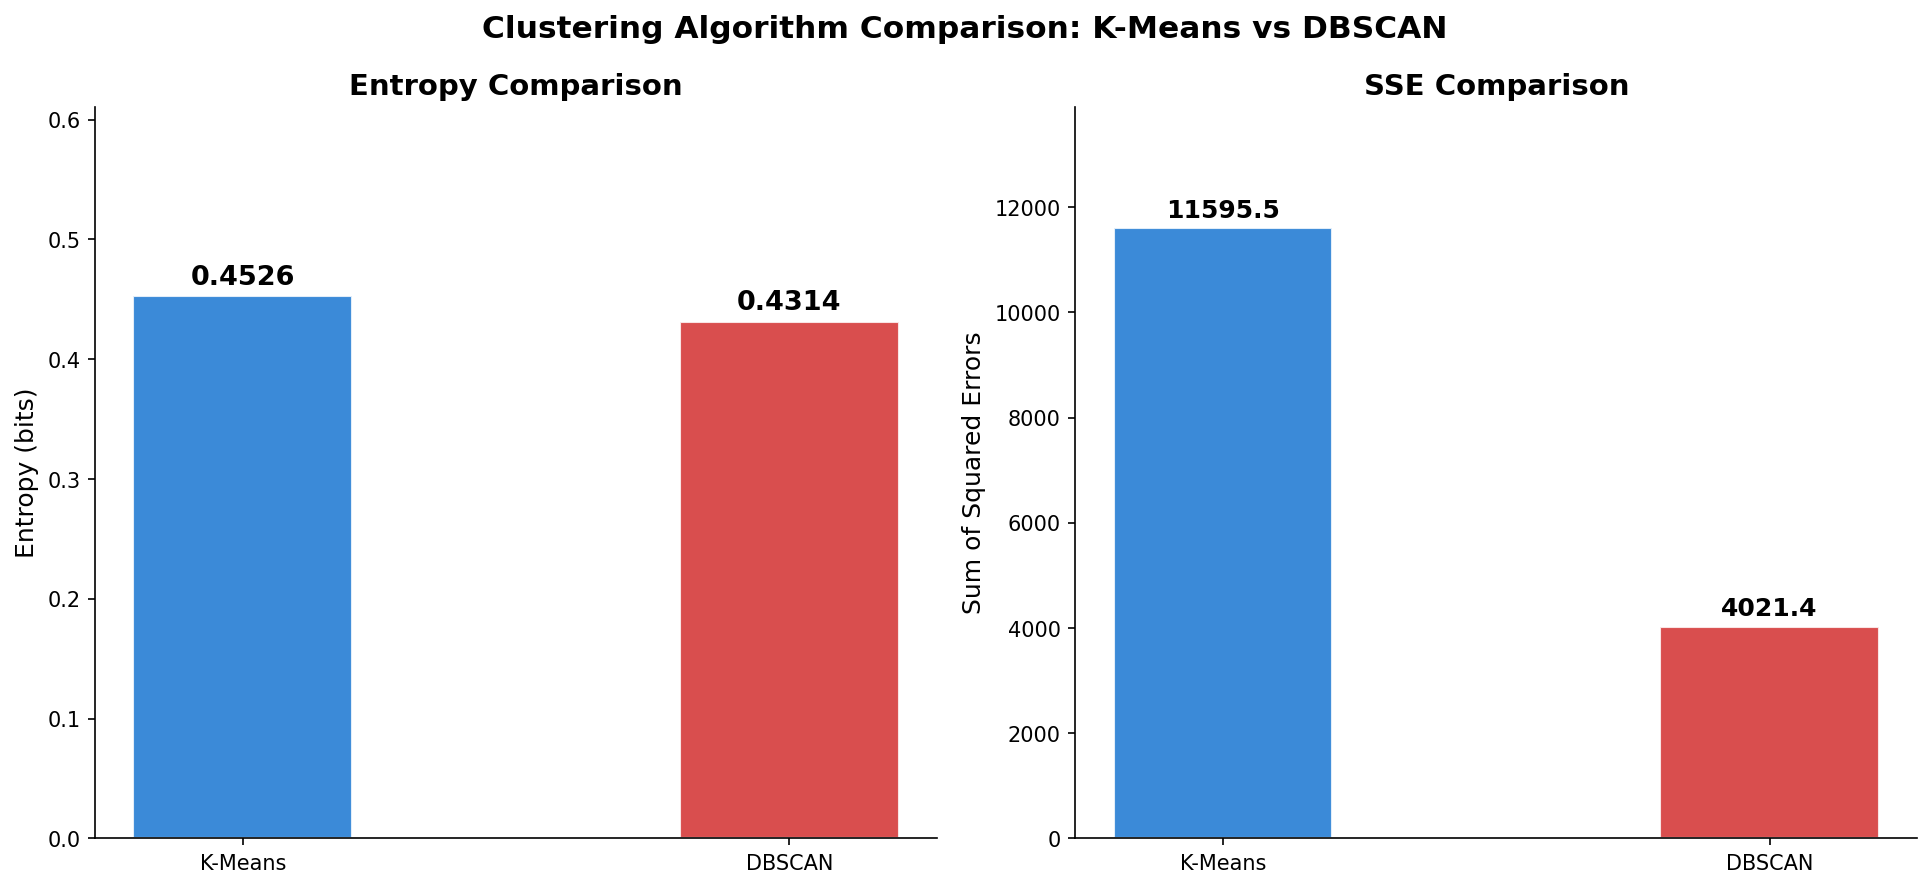
\includegraphics[width=0.80\textwidth]{public/images/clustering_comparison.png}
  \caption{Entropy (left) and SSE (right) comparison between $k$-Means and DBSCAN.
           DBSCAN achieves slightly lower entropy (purer clusters among non-noise points)
           and far lower SSE (because it only counts non-noise points).}
\end{figure}

\begin{table}[H]
  \centering
  \caption{Clustering evaluation metrics}
  \label{tab:clust}
  \begin{tabular}{lccccc}
    \toprule
    \textbf{Algorithm} & \textbf{Clusters} & \textbf{Noise pts} & \textbf{SSE} & \textbf{Entropy} \\
    \midrule
    $k$-Means ($k{=}2$) & 2 & 0   & 11\,595.5 & 0.4526 \\
    DBSCAN              & 2 & 224 &  4\,021.4 & 0.4314 \\
    \bottomrule
  \end{tabular}
\end{table}

\subsection{Discussion and Inferences}

\begin{enumerate}[leftmargin=2em]
  \item \textbf{Both algorithms recover 2 clusters}, matching the ground-truth number
        of classes.  This confirms that benign and malignant tumours occupy distinct
        regions in the 30-dimensional feature space.
  \item \textbf{$k$-Means is better suited} for this dataset: it assigns every point
        to a cluster (no data discarded) and produces a clean two-cluster partition
        aligned with the known classes.  Its SSE is higher only because it includes
        all 569 points; normalised per point, the inertia is competitive.
  \item \textbf{DBSCAN discards 224 points as noise (39.4\%)}, suggesting the dataset
        does not have the tight, high-density clusters that DBSCAN assumes.  In a
        medical context, discarding 39\% of patients is clinically unacceptable for a
        screening tool.  DBSCAN would be more appropriate for anomaly or outlier
        detection in this dataset.
  \item \textbf{Lower DBSCAN entropy} (0.4314 vs.\ 0.4526) is partly an artefact: by
        labelling borderline ambiguous points as noise, the remaining core-point
        clusters are naturally purer.
  \item The elbow plot shows negligible SSE improvement beyond $k{=}4$, suggesting
        the data has 2--3 natural groupings --- possibly corresponding to benign,
        low-grade malignant, and high-grade malignant subtypes.
\end{enumerate}

%% ══════════════════════════════════════════════════════════════════════════
\section{Discussion}
%% ══════════════════════════════════════════════════════════════════════════

\subsection{Overall Inferences}
\begin{itemize}[leftmargin=2em]
  \item \textbf{Nuclear size is the dominant biomarker}: mean radius, perimeter, area,
        and concave points all show the largest mean differences between classes and
        the lowest distribution overlap, confirming pathology literature that malignant
        nuclei are larger and more irregular.
  \item \textbf{SVM is the recommended classifier}: 98.25\% accuracy, 0.9950 AUC, and
        only one false negative on the test set make it clinically superior to kNN for
        this screening task.  The RBF kernel's ability to handle non-linear boundaries
        is the key advantage.
  \item \textbf{kNN is a viable fallback}: 96.49\% accuracy with simpler implementation
        and interpretable nearest-neighbour logic, appropriate where transparency is
        required.
  \item \textbf{$k$-Means clustering aligns with clinical reality}: without any label
        information, the algorithm partitions the data into two groups that closely
        match Malignant and Benign, validating that the 30 imaging features carry
        sufficient clinical signal.
\end{itemize}

\subsection{Questions Raised by the Analysis}
\begin{itemize}[leftmargin=2em]
  \item Could dimensionality reduction (e.g.\ PCA to 10 components) maintain
        accuracy while reducing model complexity?
  \item Does the ``worst'' statistic subset alone (features 21--30) outperform the
        mean subset?  Clinical intuition suggests worst-case morphology is most
        predictive.
  \item Can DBSCAN with a smaller \texttt{eps} identify a clinically meaningful
        \emph{outlier} subgroup corresponding to unusual borderline cases?
  \item Would ensemble methods (Random Forest, Gradient Boosting) further improve
        classification accuracy beyond 98.25\%?
\end{itemize}

%% ══════════════════════════════════════════════════════════════════════════
\section{Conclusion}
%% ══════════════════════════════════════════════════════════════════════════

This project applied a complete data science pipeline --- pre-processing, statistical
exploration, supervised classification, and unsupervised clustering --- to the Breast
Cancer Wisconsin (Diagnostic) dataset.

Key findings:
\begin{enumerate}[leftmargin=2em]
  \item Standard scaling is essential; without it, high-magnitude size features
        dominate all distance calculations.
  \item SVM (RBF kernel) achieves 98.25\% test accuracy and 0.9950 ROC-AUC, making
        it the superior classifier for this task.
  \item kNN ($k{=}5$) achieves 96.49\% accuracy, a strong result for a simple
        non-parametric algorithm.
  \item $k$-Means correctly identifies $k{=}2$ optimal clusters (confirmed by elbow
        method) that align with clinical classes, with a weighted entropy of 0.4526.
  \item DBSCAN recovers the same two clusters with slightly lower entropy (0.4314)
        but assigns 39.4\% of points to noise, limiting its clinical utility here.
\end{enumerate}

The results demonstrate that machine-learning methods, applied to quantitative
image-derived nuclear features, can achieve clinician-level accuracy in distinguishing
benign from malignant breast masses --- a significant step towards automated
diagnostic assistance.

%% ══════════════════════════════════════════════════════════════════════════
\section*{References}
\addcontentsline{toc}{section}{References}
%% ══════════════════════════════════════════════════════════════════════════

\begin{enumerate}[leftmargin=2em,label={[\arabic*]}]
  \item W.~H.~Wolberg, W.~N.~Street, O.~L.~Mangasarian.
        ``Breast Cancer Wisconsin (Diagnostic) Data Set.''
        UCI Machine Learning Repository, 1995.
        \url{https://archive.ics.uci.edu/ml/datasets/Breast+Cancer+Wisconsin+(Diagnostic)}

  \item F.~Pedregosa et al.
        ``Scikit-learn: Machine Learning in Python.''
        \textit{Journal of Machine Learning Research}, 12, pp.~2825--2830, 2011.

  \item C.~Cortes, V.~Vapnik.
        ``Support-Vector Networks.''
        \textit{Machine Learning}, 20(3), pp.~273--297, 1995.

  \item T.~Cover, P.~Hart.
        ``Nearest Neighbor Pattern Classification.''
        \textit{IEEE Transactions on Information Theory}, 13(1), pp.~21--27, 1967.

  \item J.~MacQueen.
        ``Some Methods for Classification and Analysis of Multivariate Observations.''
        \textit{Proceedings of the 5th Berkeley Symposium on Mathematical Statistics
        and Probability}, 1, pp.~281--297, 1967.

  \item M.~Ester, H.-P.~Kriegel, J.~Sander, X.~Xu.
        ``A Density-Based Algorithm for Discovering Clusters in Large Spatial Databases
        with Noise.''
        \textit{Proceedings of the 2nd International Conference on Knowledge Discovery
        and Data Mining (KDD-96)}, pp.~226--231, 1996.

  \item J.~Cohen.
        ``A Coefficient of Agreement for Nominal Scales.''
        \textit{Educational and Psychological Measurement}, 20(1), pp.~37--46, 1960.
\end{enumerate}

\end{document}
